\documentclass{scrreprt}

\usepackage[utf8]{inputenc} % Paket zum Erkennen deutscher Umlaute
\usepackage[T1]{fontenc} % Ansonst wir ein ä als a mit 2 Punkten anstelle eines ä angezeigt
% Alternativ: Umlaute \"a \"o \"u  Mit Leerzeichen \ss{} nach dem Zeichen

%\usepackage{ngerman} %Paket für deutsche Rechtschreibung
% Alternativ:
\usepackage[ngerman]{babel}
\usepackage{ngerman,graphicx}



\usepackage{setspace} %Paket zum Ändern des Zeilenabstandes
%\onehalfspacing
%\doublespacing

\linespread{1.5}

\author{Fabian Konrad, Armin Beck, André Berberich}
\title{Unterschiedliche Datenkapazität bei CDs und DVDs}


\begin{document}
\maketitle
\newpage

\chapter{Versuch zur Bestimmung des Spurabstands einer CD und einer DVD}



\section{Einleitung}
Unterschiedliche Speicherkapazität von CD / DVD bei gleicher Baugröße
Allgemeine Verbreitung
Als Phillips und Sony Ende der Siebzigerjahre des letzten Jahrtausends die CD entwickelten, war bereits vorauszusehen, dass dieses Medium alle seine Vorgänger in den Schatten stellen würde. Man hatte auf dem Gebiet der Tontechnik eine komplette Revolution vorangetrieben. Die CD war stabiler als ihre Vorgänger, sie vertrug weitaus größere Beschädigungen und ihre Qualität ist auch wenn der Datenträger bereits zwanzig Jahre alt ist immer noch die selbe wie zu Beginn. Der Grund dafür ist, dass die Compact Disc, wie man sie auch nennt, das erste weit verbreitete Medium für Musik und Ton ist, auf dem die Daten in digitaler Form gespeichert sind. Außerdem ist sie das erste auf dem Markt, das ein optisches Leseverfahren verwendet. In Tausenden Ringen im Mikrometerabstand sind winzige Löcher auf eine Kunststoffplatte geprägt, die die binären Daten darstellen. Diese Daten können durch Spiegelung eines Lasersignals gelesen werden. Wenn man sie nun an einen Decoder schickt, der daraus analoge Schallsignale entstehen lässt, erhält man letztendlich die auf der CD gespeicherten Tonsignale. Bei einer DVD wird genau dasselbe Verfahren angewendet. Allerdings ist der Abstand und folglich auch der Flächenverbrauch je Loch hier deutlich geringer, somit steigt die Datenkapazität auf das Fünffache an. Es besteht des Weiteren die Möglichkeit, bis zu 2 Schichten übereinander zu legen und zu lesen. Dies verdoppelt die Datenkapazität wiederum. Da der Lochabstand von CD und DVD extrem gering ist, kann man diese mit einem handelsüblichen Laserpointer durchleuchten und hierbei die Löcher als Doppelspalt verwenden. Es treten die für einen Doppelspalt typischen Effekte auf, anhand deren man das Verhältnis aus Wellenlänge und Lochabstand berechnen kann.


\section{Interferenz}
Überlagerung von Wellen zur Feststellung der Abstände
Unterscheidet sich vom Leseverfahren welches eine ledigliche Spiegelung ist
Grundlagen/Hinführung wieso Laser verwendet wurde

\section{Aufbau und Lese-/Schreibverfahren einer CD und einer DVD}Vergleich CD / DVD

\begin{figure}[!htbp]
\centering
\includegraphics[width=0.6\textwidth,keepaspectratio]{Pictures/DiskCD.png}
\parbox{0.9\textwidth}

{\caption{\label{fig:CD1}
Laser CD}
\sffamily \small{Schnittzeichnung der Strahlgeometrie bei einer CD}
}
\end{figure}



\begin{figure}[!htbp]
\centering
\includegraphics[width=0.6\textwidth,keepaspectratio]{Pictures/DiskDVD.png}
\parbox{0.9\textwidth}

{\caption{\label{fig:DVD1}
Laser DVD}
\sffamily \small{Schnittzeichnung der Strahlgeometrie bei einer DVD}
}
\end{figure}

\section{Versuchsaufbau}
\begin{figure}[!htbp]
\centering
\includegraphics[width=0.6\textwidth,keepaspectratio]
{Pictures/Versuchsaufbau.png}
\parbox{0.9\textwidth}

{\caption{\label{fig:Versuchsaufbau}
Schematischer Aufbau}
\sffamily \small{Versuchsaufbau}
}
\end{figure}

\section{Versuchsergebnisse}
Diagramm, Tabelle mit Messwerte, Bilder der Versuchsdurchführung

\section{Fehleranalyse}
Darstellung möglicher Fehlerquellen ( Laborbedingungen, Toleranzen, Messungenauigkeit)
\section{Interpretation / Fazit}
Einschätzung Versuchsaufbau (wie zielführend war der Versuch?)




\bibliographystyle{unsrt} 
% Stil sollte \bibliographystyle{harvard} da von der DHBW "empfohlen"
 \bibliography{ReferenceDatabase} %Pfadangabe zur Zitatdatei

\listoffigures

\chapter{PlaceHolder Citation}

Zitat Eichler \cite{Eichler2015}

Zitat Reider \cite{Reider2012}

\chapter{PlaceHolder Pictures}



\begin{figure}[!htbp]
\centering
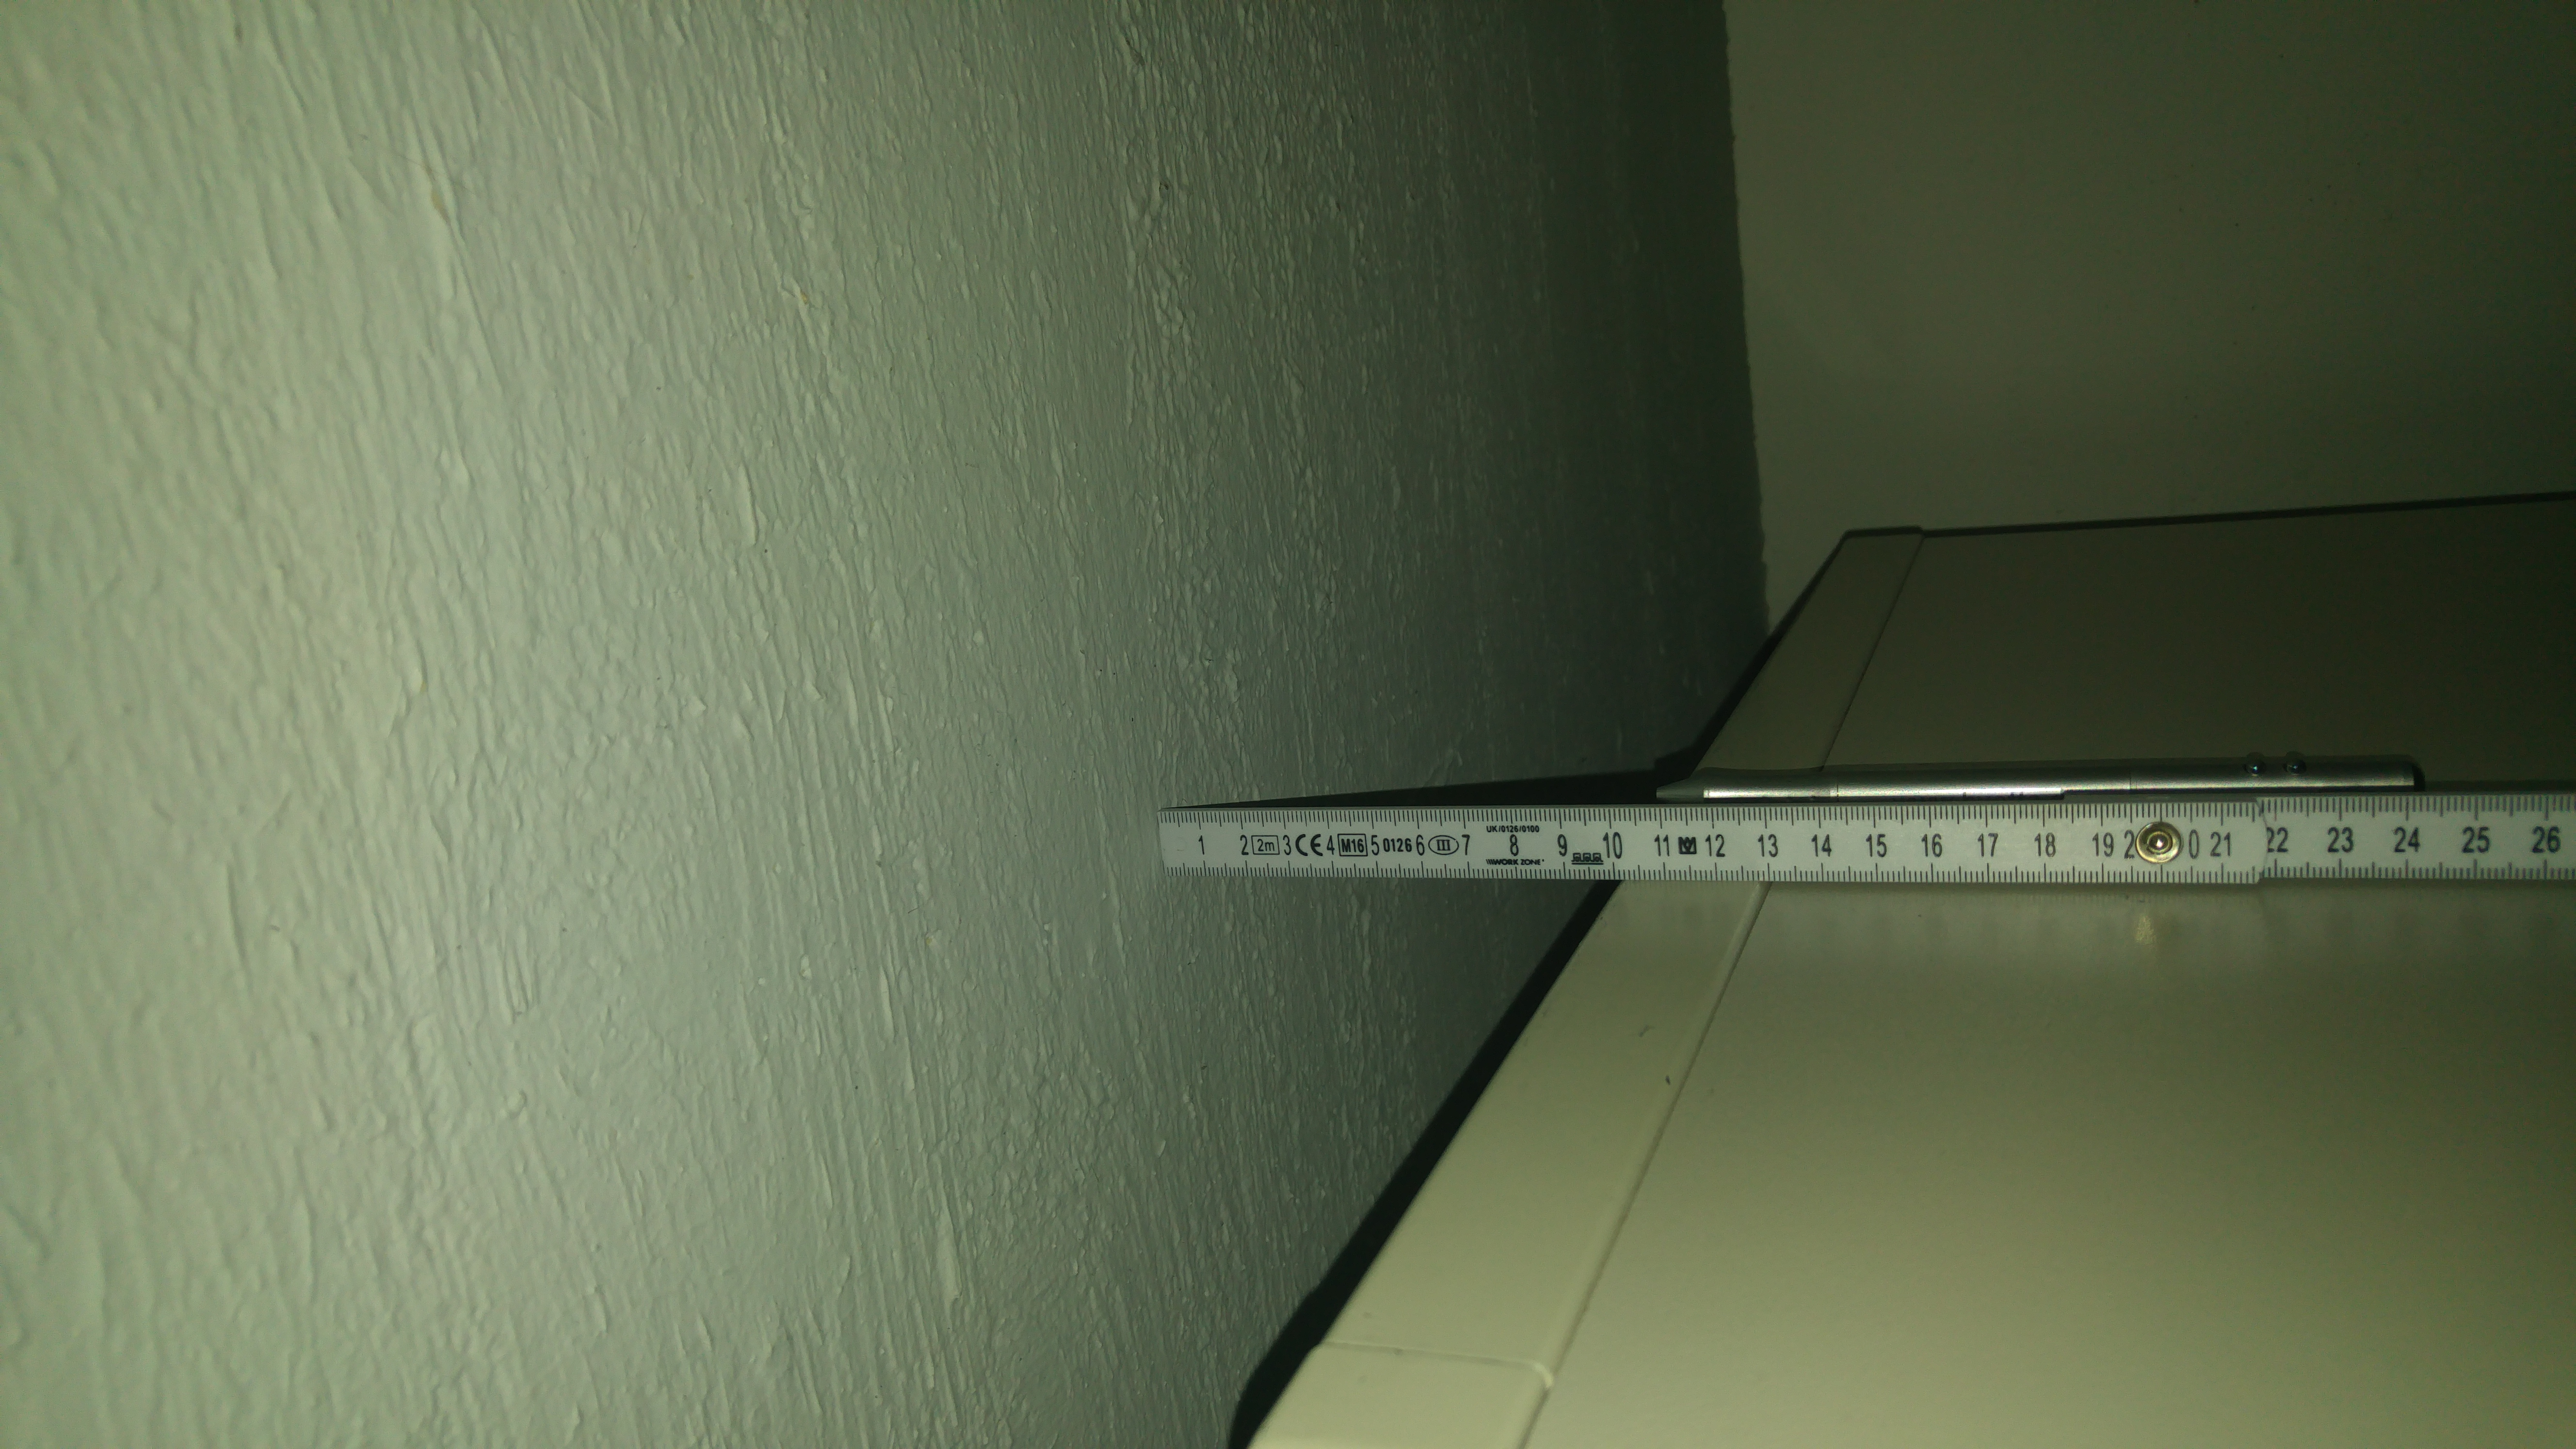
\includegraphics[width=0.6\textwidth,keepaspectratio]
{Pictures/20161219_140859.jpg}
\parbox{0.9\textwidth}

{\caption{\label{fig:Bild1}
Bildtitel für Bild 1}
\sffamily \small{Beschreibung für Bild 1}
}
\end{figure}

\begin{figure}[!htbp]
\centering
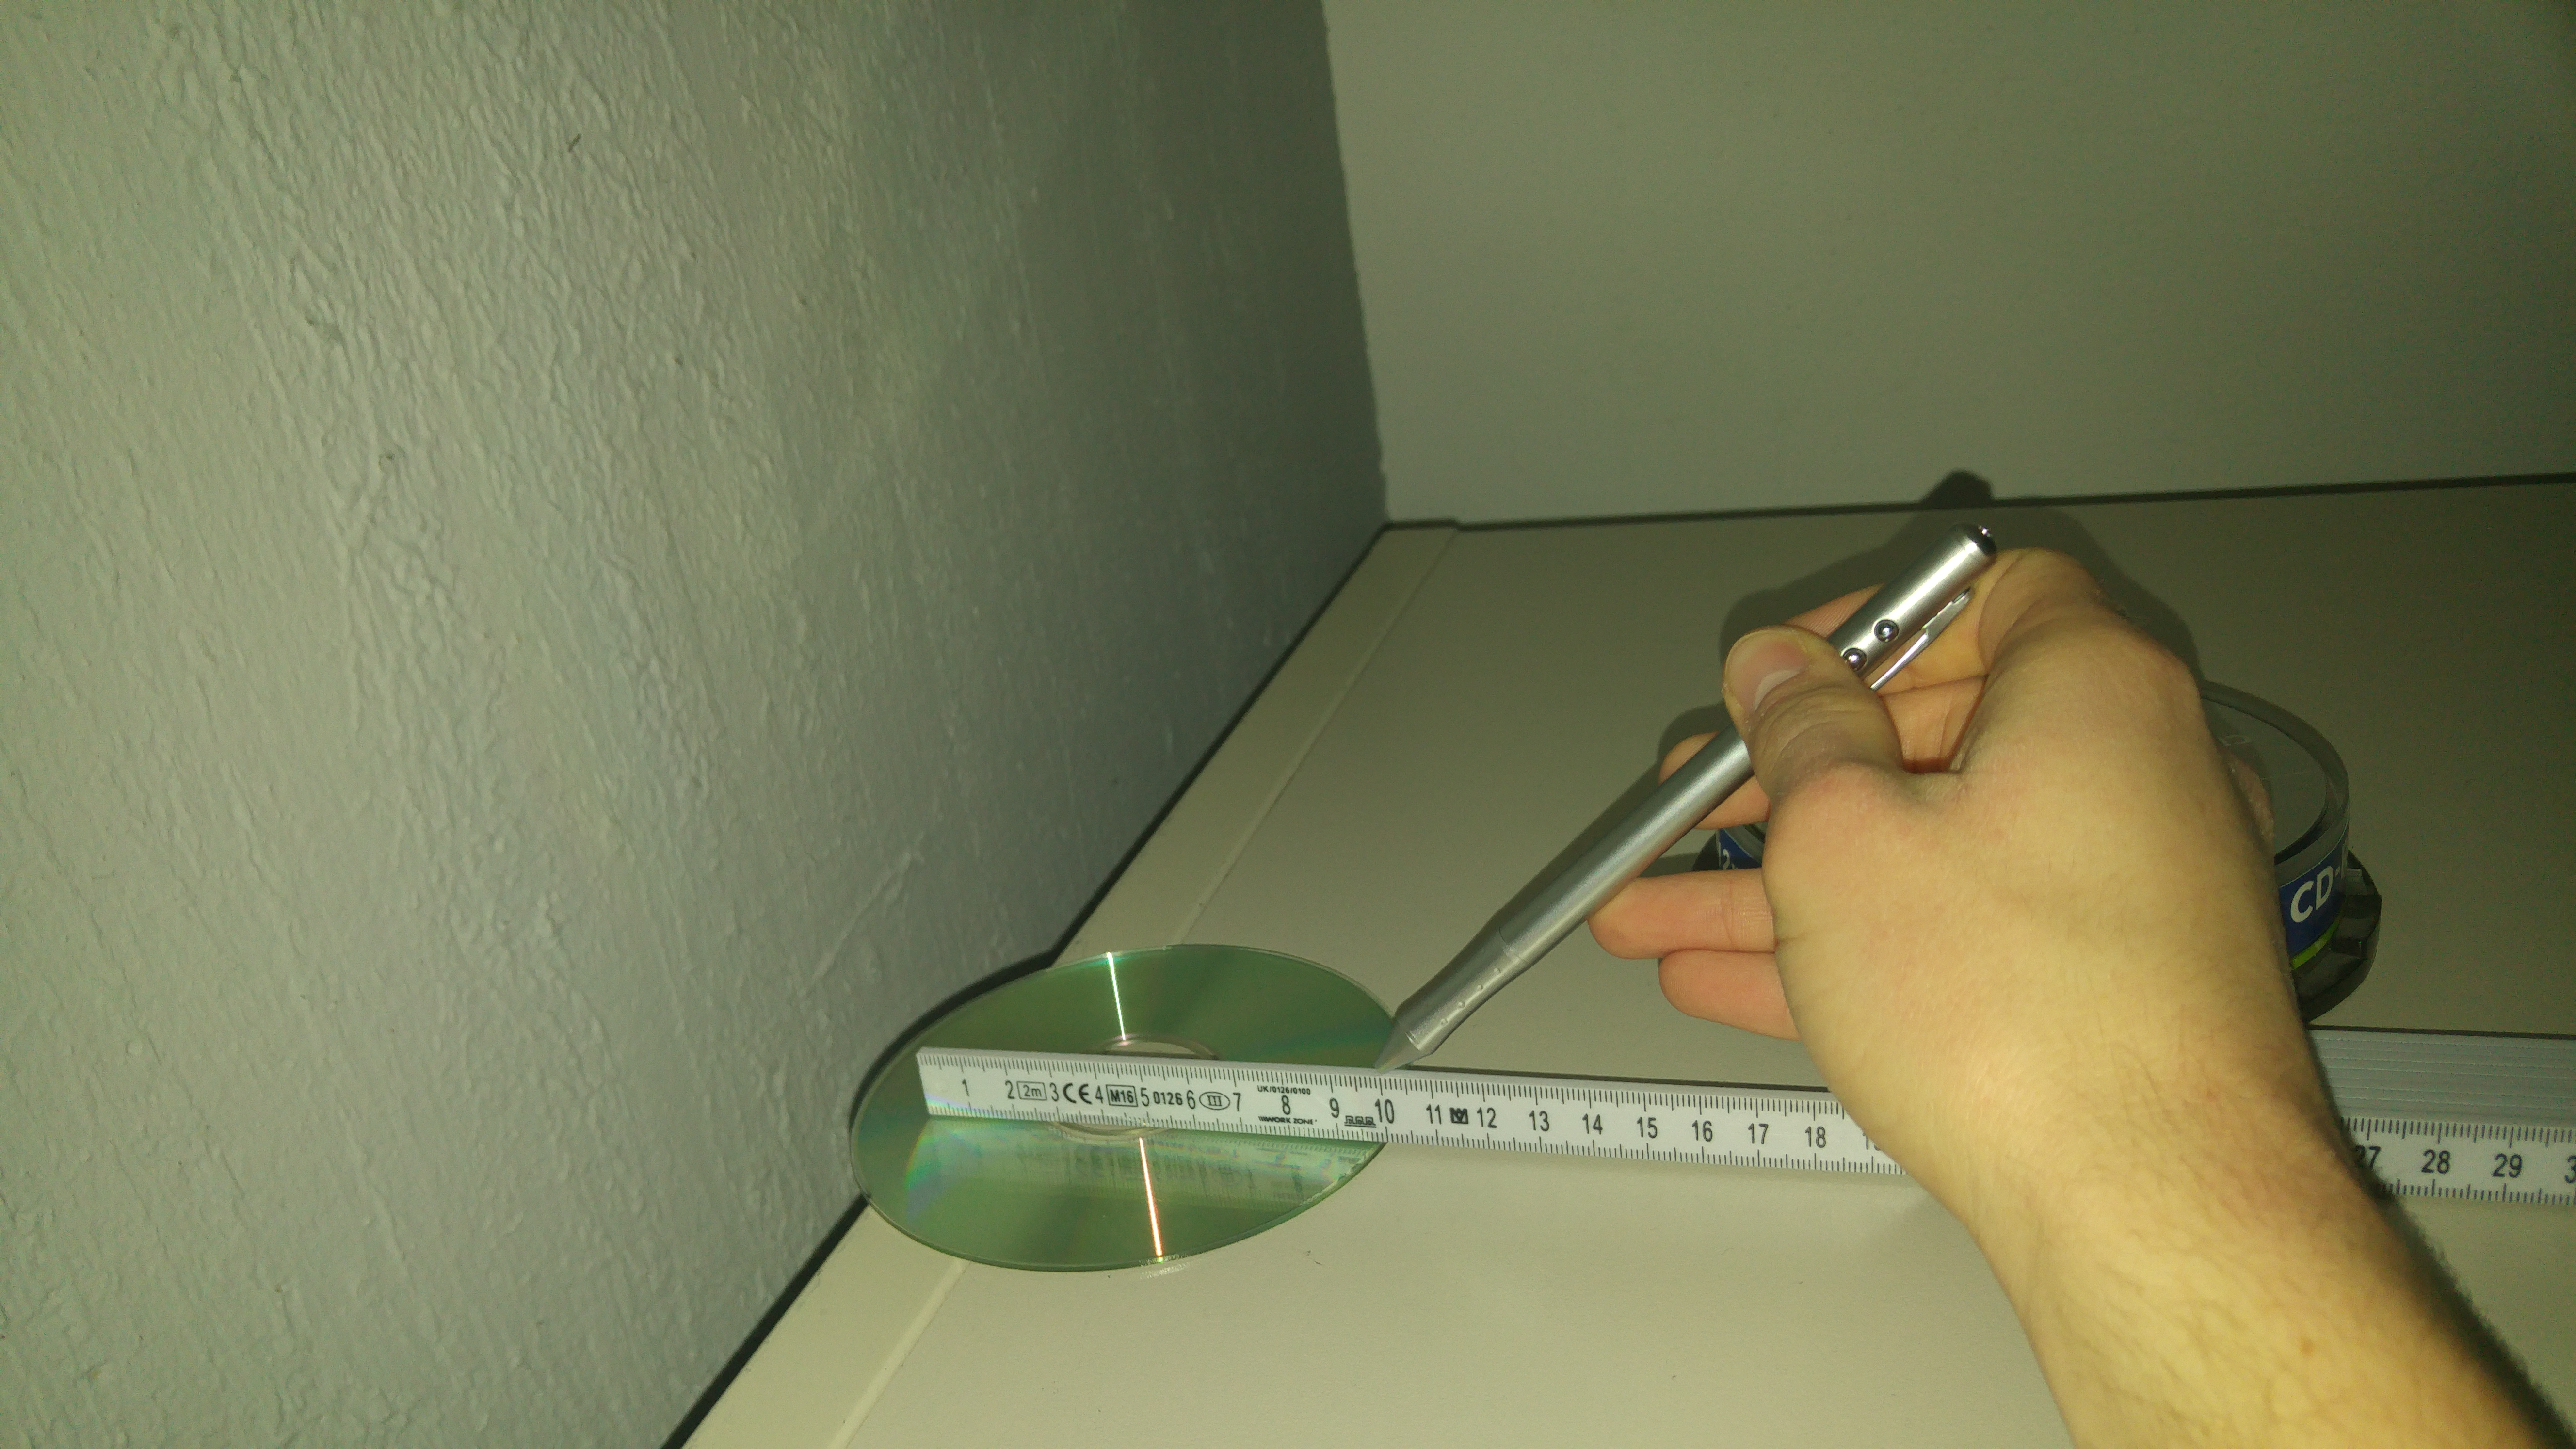
\includegraphics[width=0.6\textwidth,keepaspectratio]
{Pictures/20161219_141254.jpg}
\parbox{0.9\textwidth}

{\caption{\label{fig:Bild2}
Bildtitel für Bild 2}
\sffamily \small{Beschreibung für Bild 2}
}
\end{figure}

\begin{figure}[!htbp]
\centering
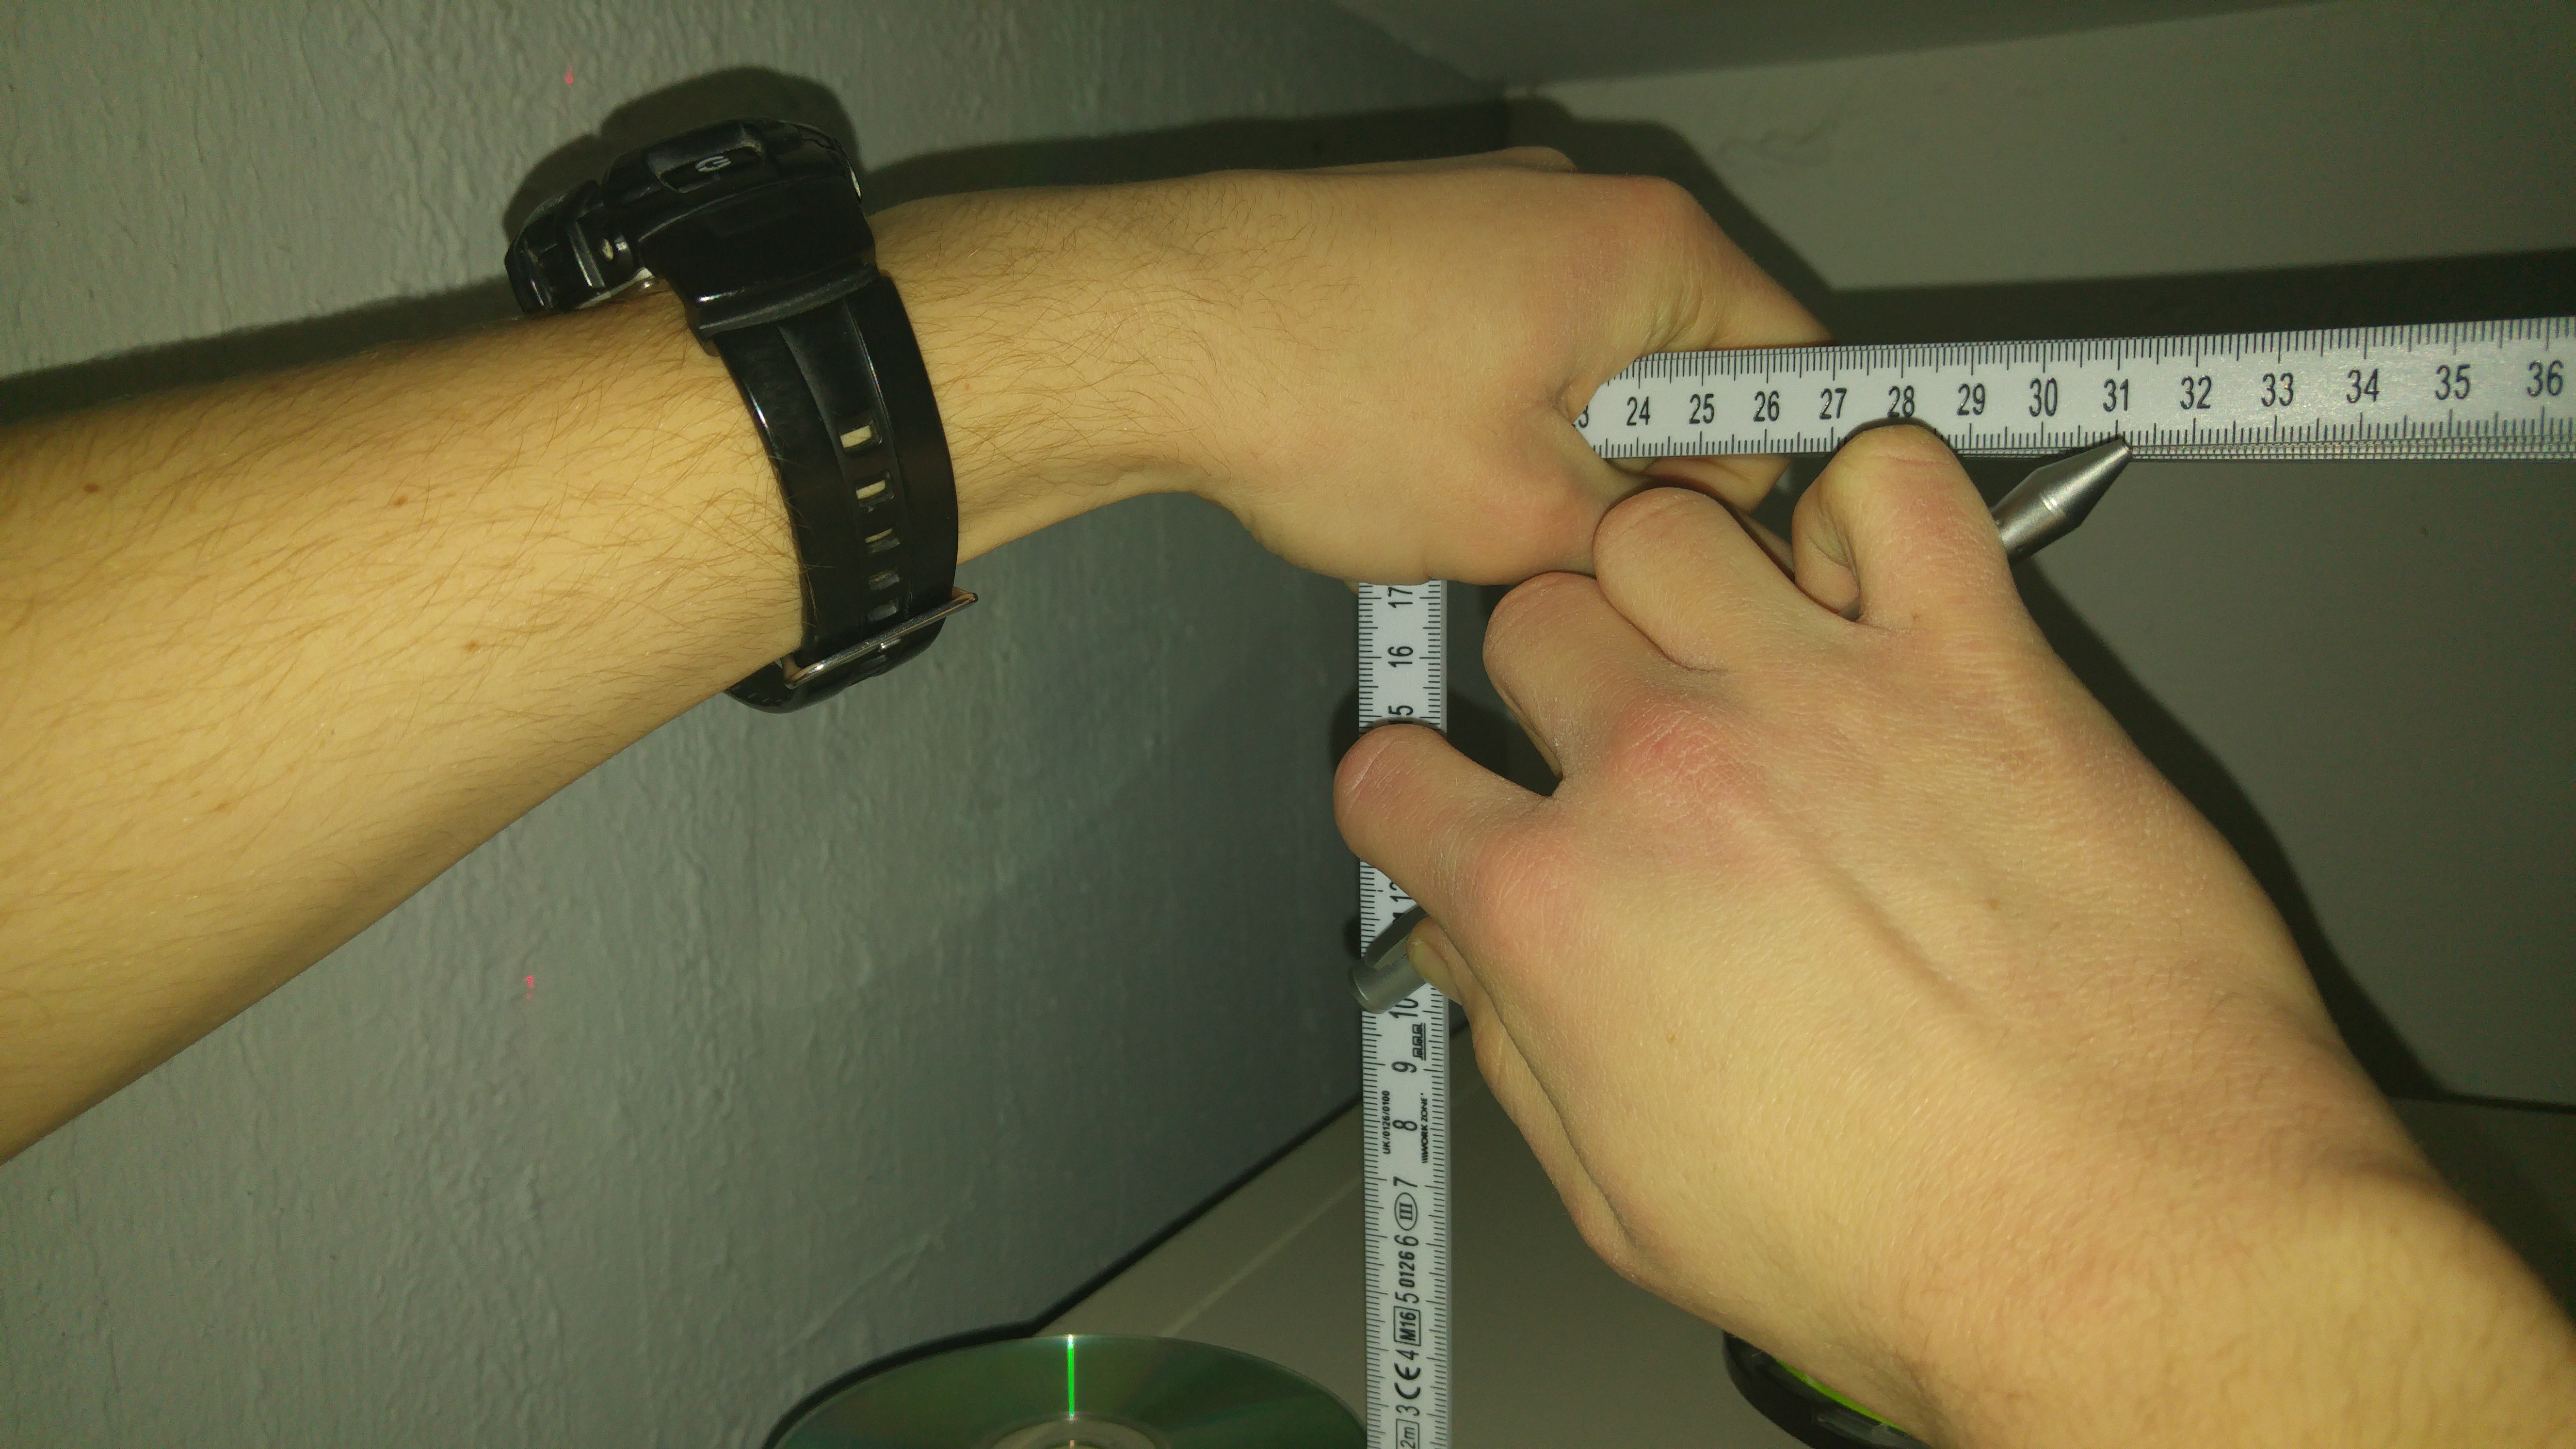
\includegraphics[width=0.6\textwidth,keepaspectratio]
{Pictures/20161219_141516.jpg}
\parbox{0.9\textwidth}

{\caption{\label{fig:Bild3}
Bildtitel für Bild 3}
\sffamily \small{Beschreibung für Bild 3}
}
\end{figure}



\begin{figure}[!htbp]
\centering
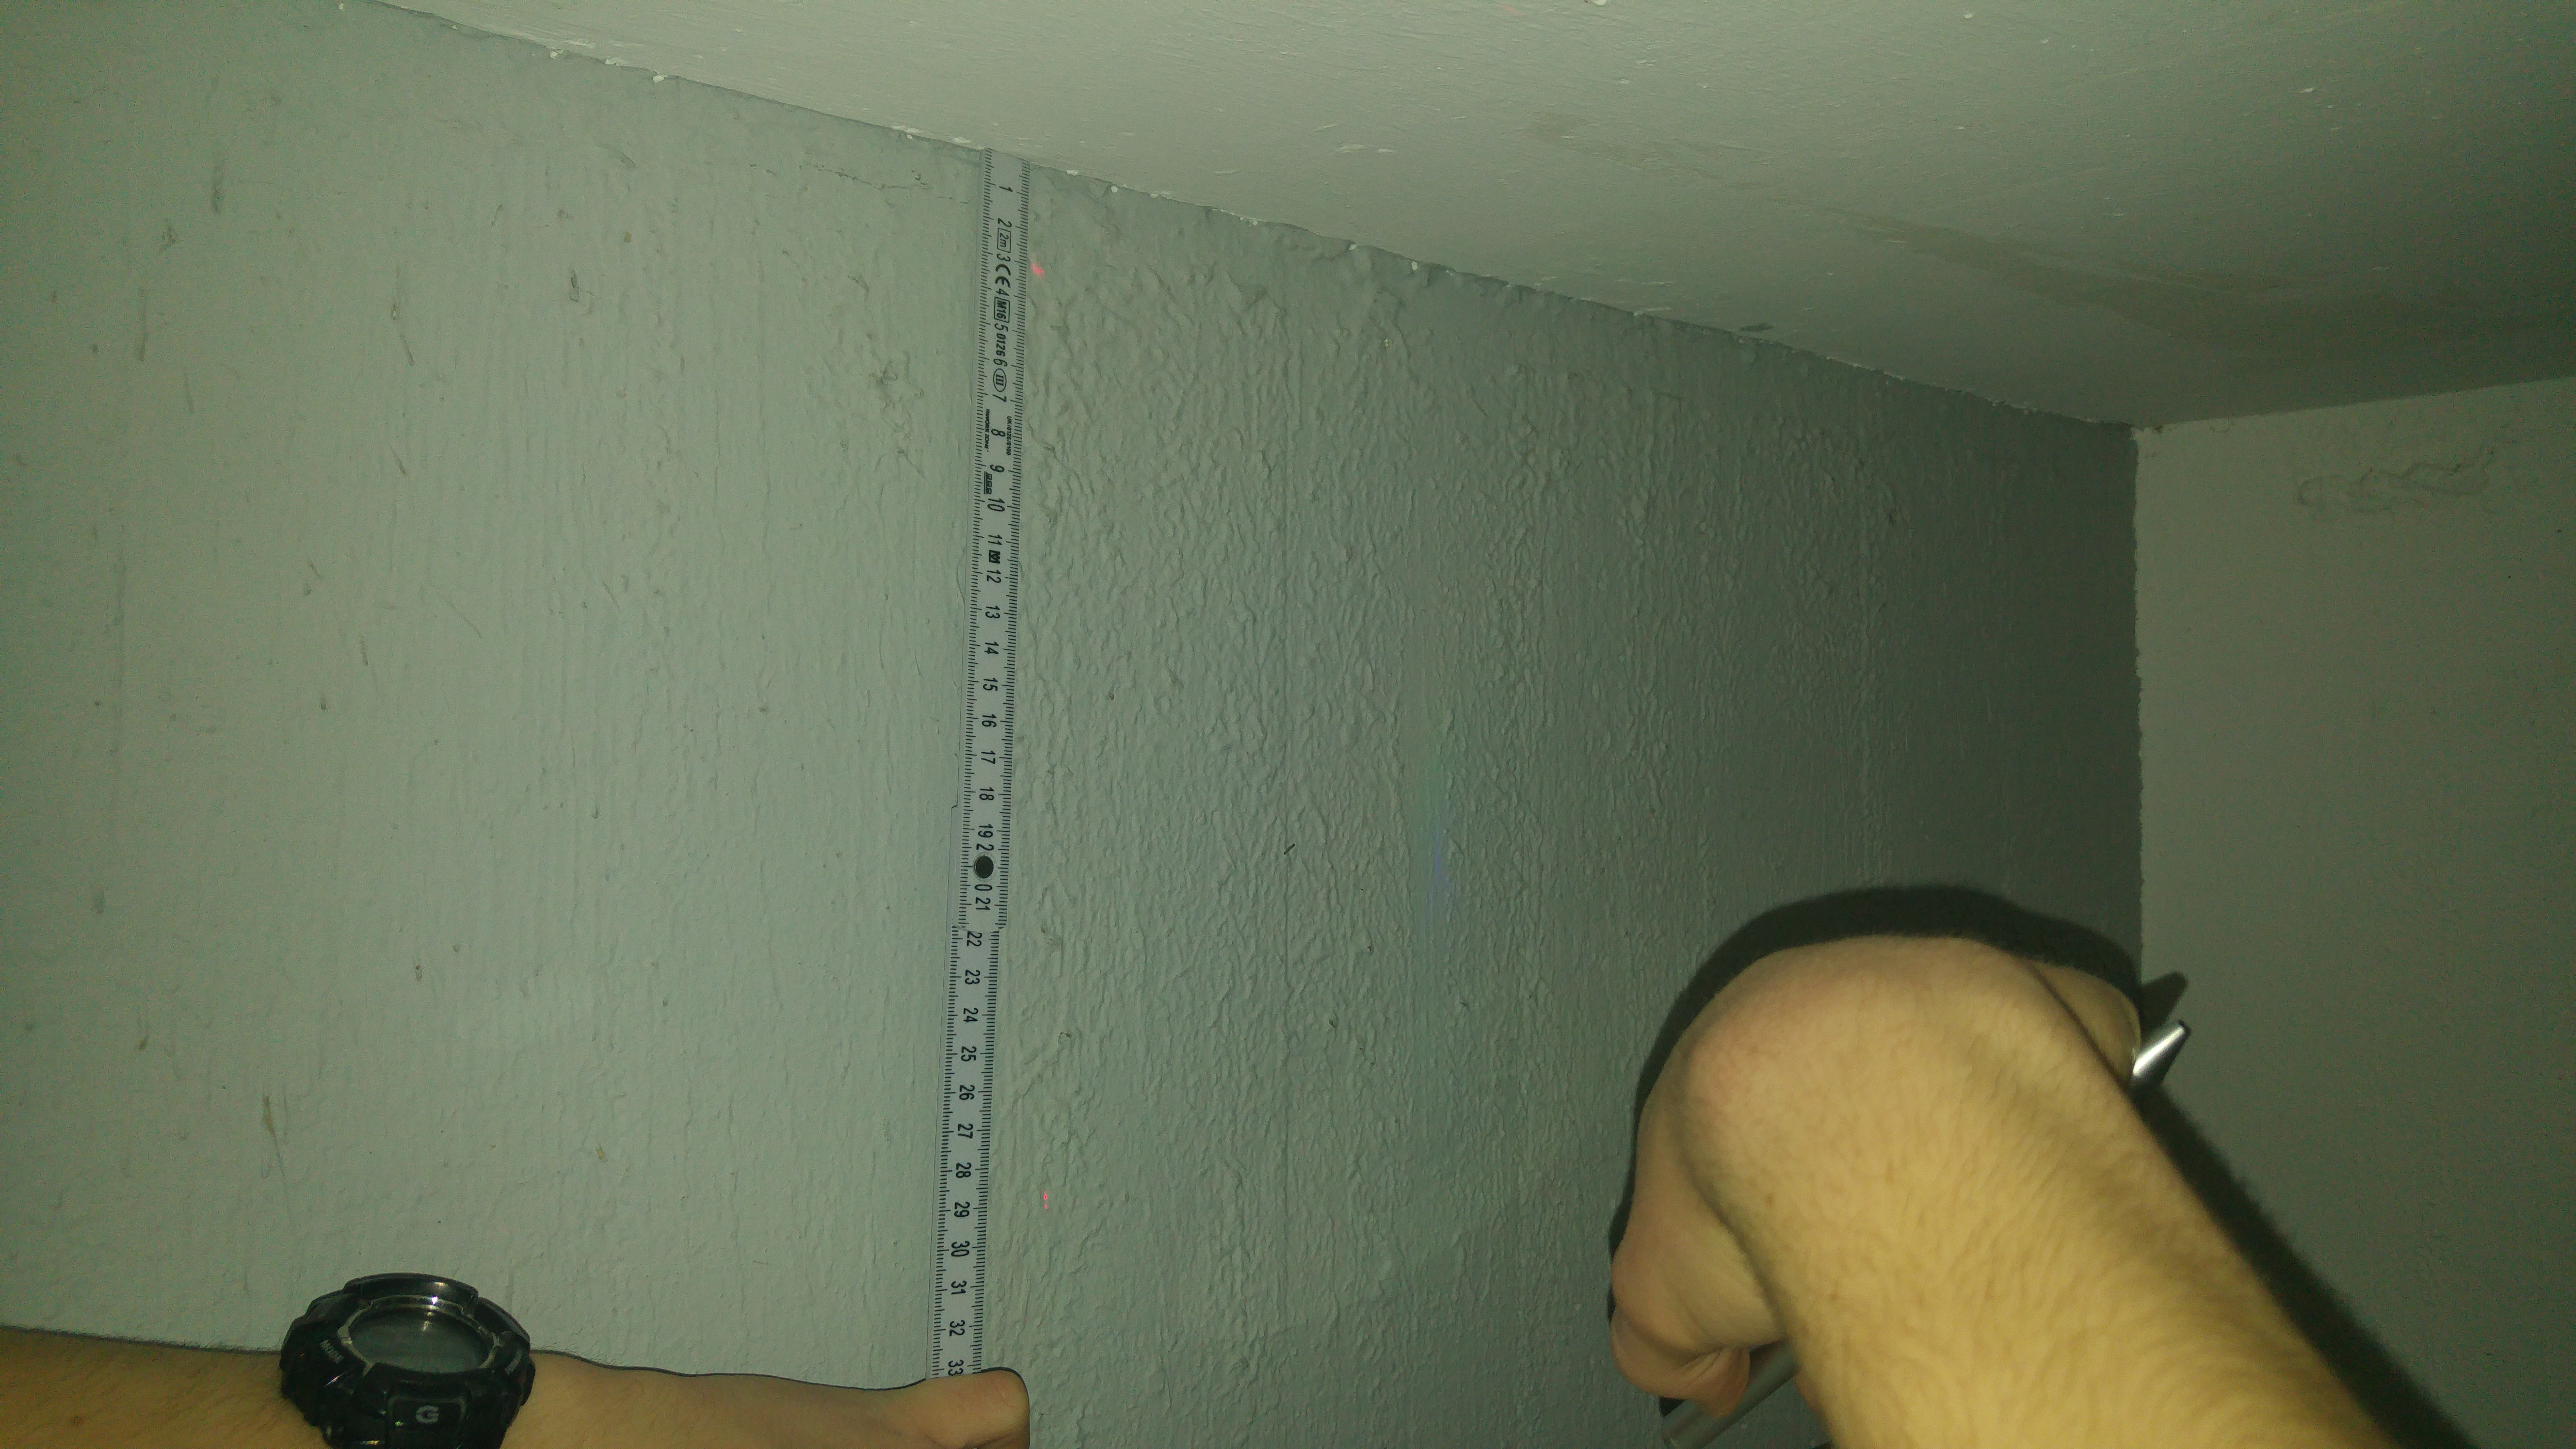
\includegraphics[width=0.6\textwidth,keepaspectratio]
{Pictures/20161219_141547.jpg}
\parbox{0.9\textwidth}

{\caption{\label{fig:Bild4}
Bildtitel für Bild 4}
\sffamily \small{Beschreibung für Bild 4}
}
\end{figure}

\begin{figure}[!htbp]
\centering
\includegraphics[width=0.6\textwidth,keepaspectratio]
{Pictures/20161219_141832.jpg}
\parbox{0.9\textwidth}

{\caption{\label{fig:Bild5}
Bildtitel für Bild 5}
\sffamily \small{Beschreibung für Bild 5}
}
\end{figure}

\begin{figure}[!htbp]
\centering
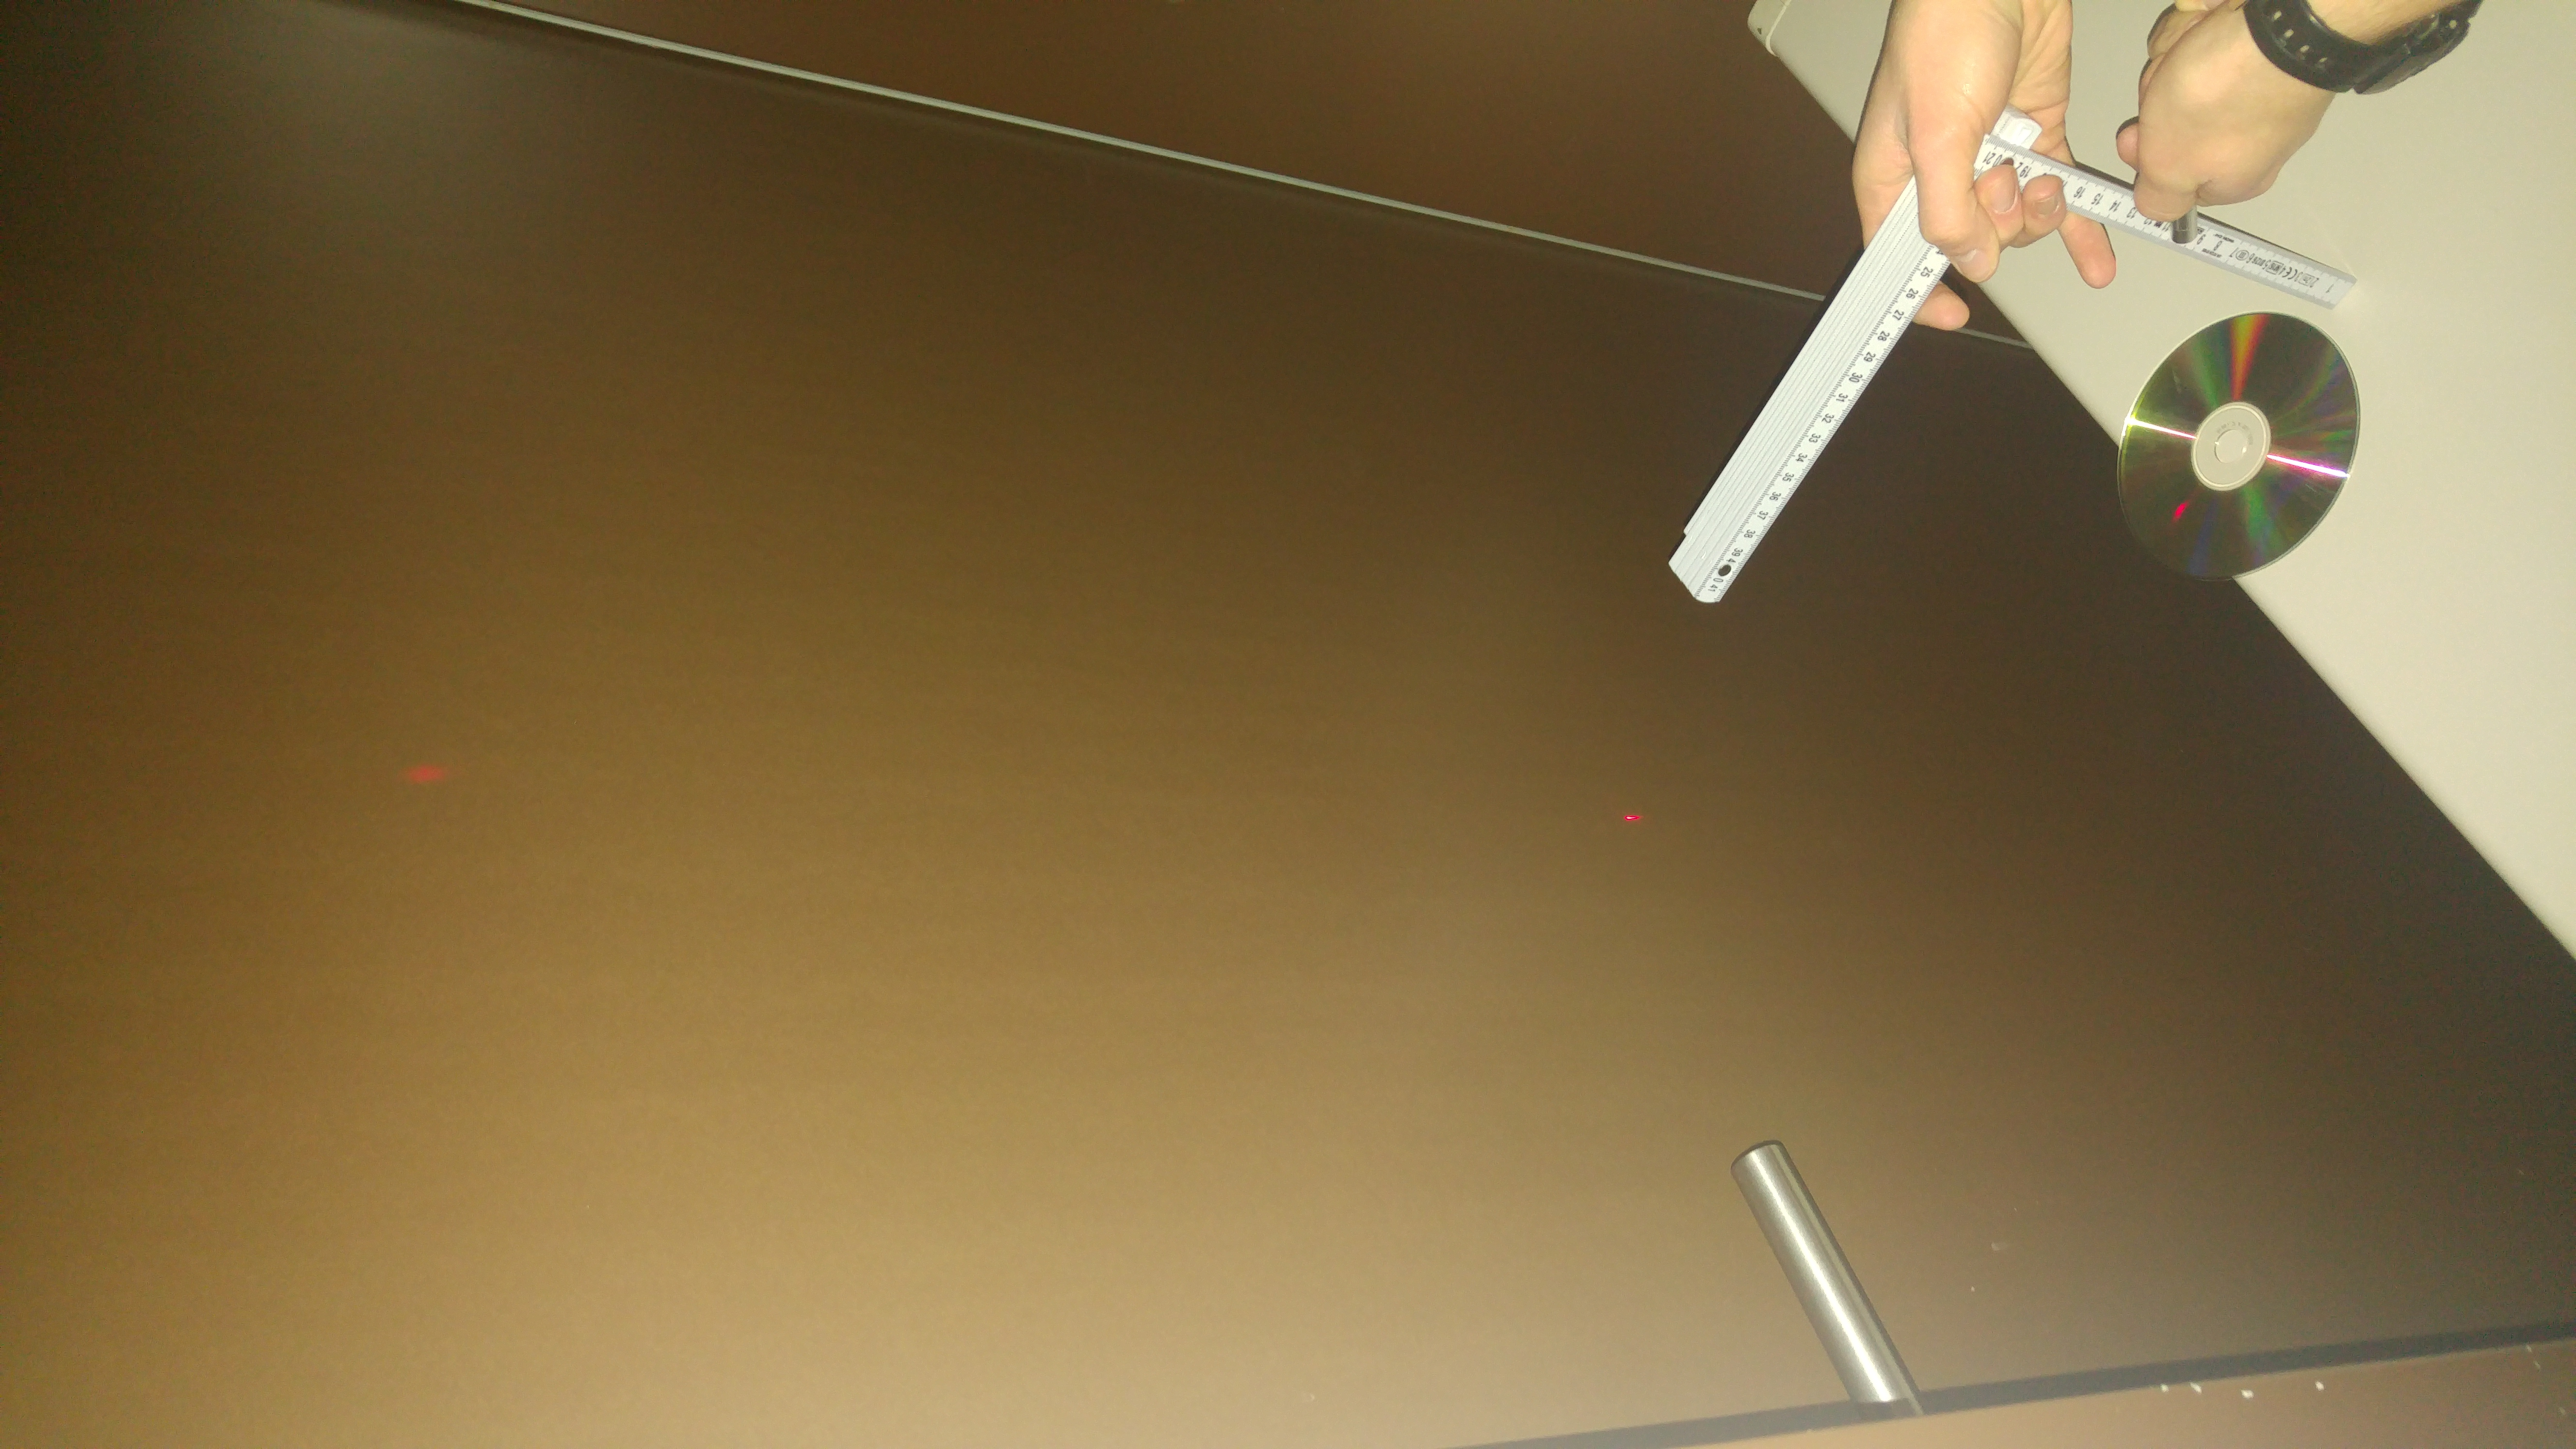
\includegraphics[width=0.6\textwidth,keepaspectratio]
{Pictures/20161219_142007.jpg}
\parbox{0.9\textwidth}

{\caption{\label{fig:Bild6}
Bildtitel für Bild 6}
\sffamily \small{Beschreibung für Bild 6}
}
\end{figure}

\begin{figure}[!htbp]
\centering
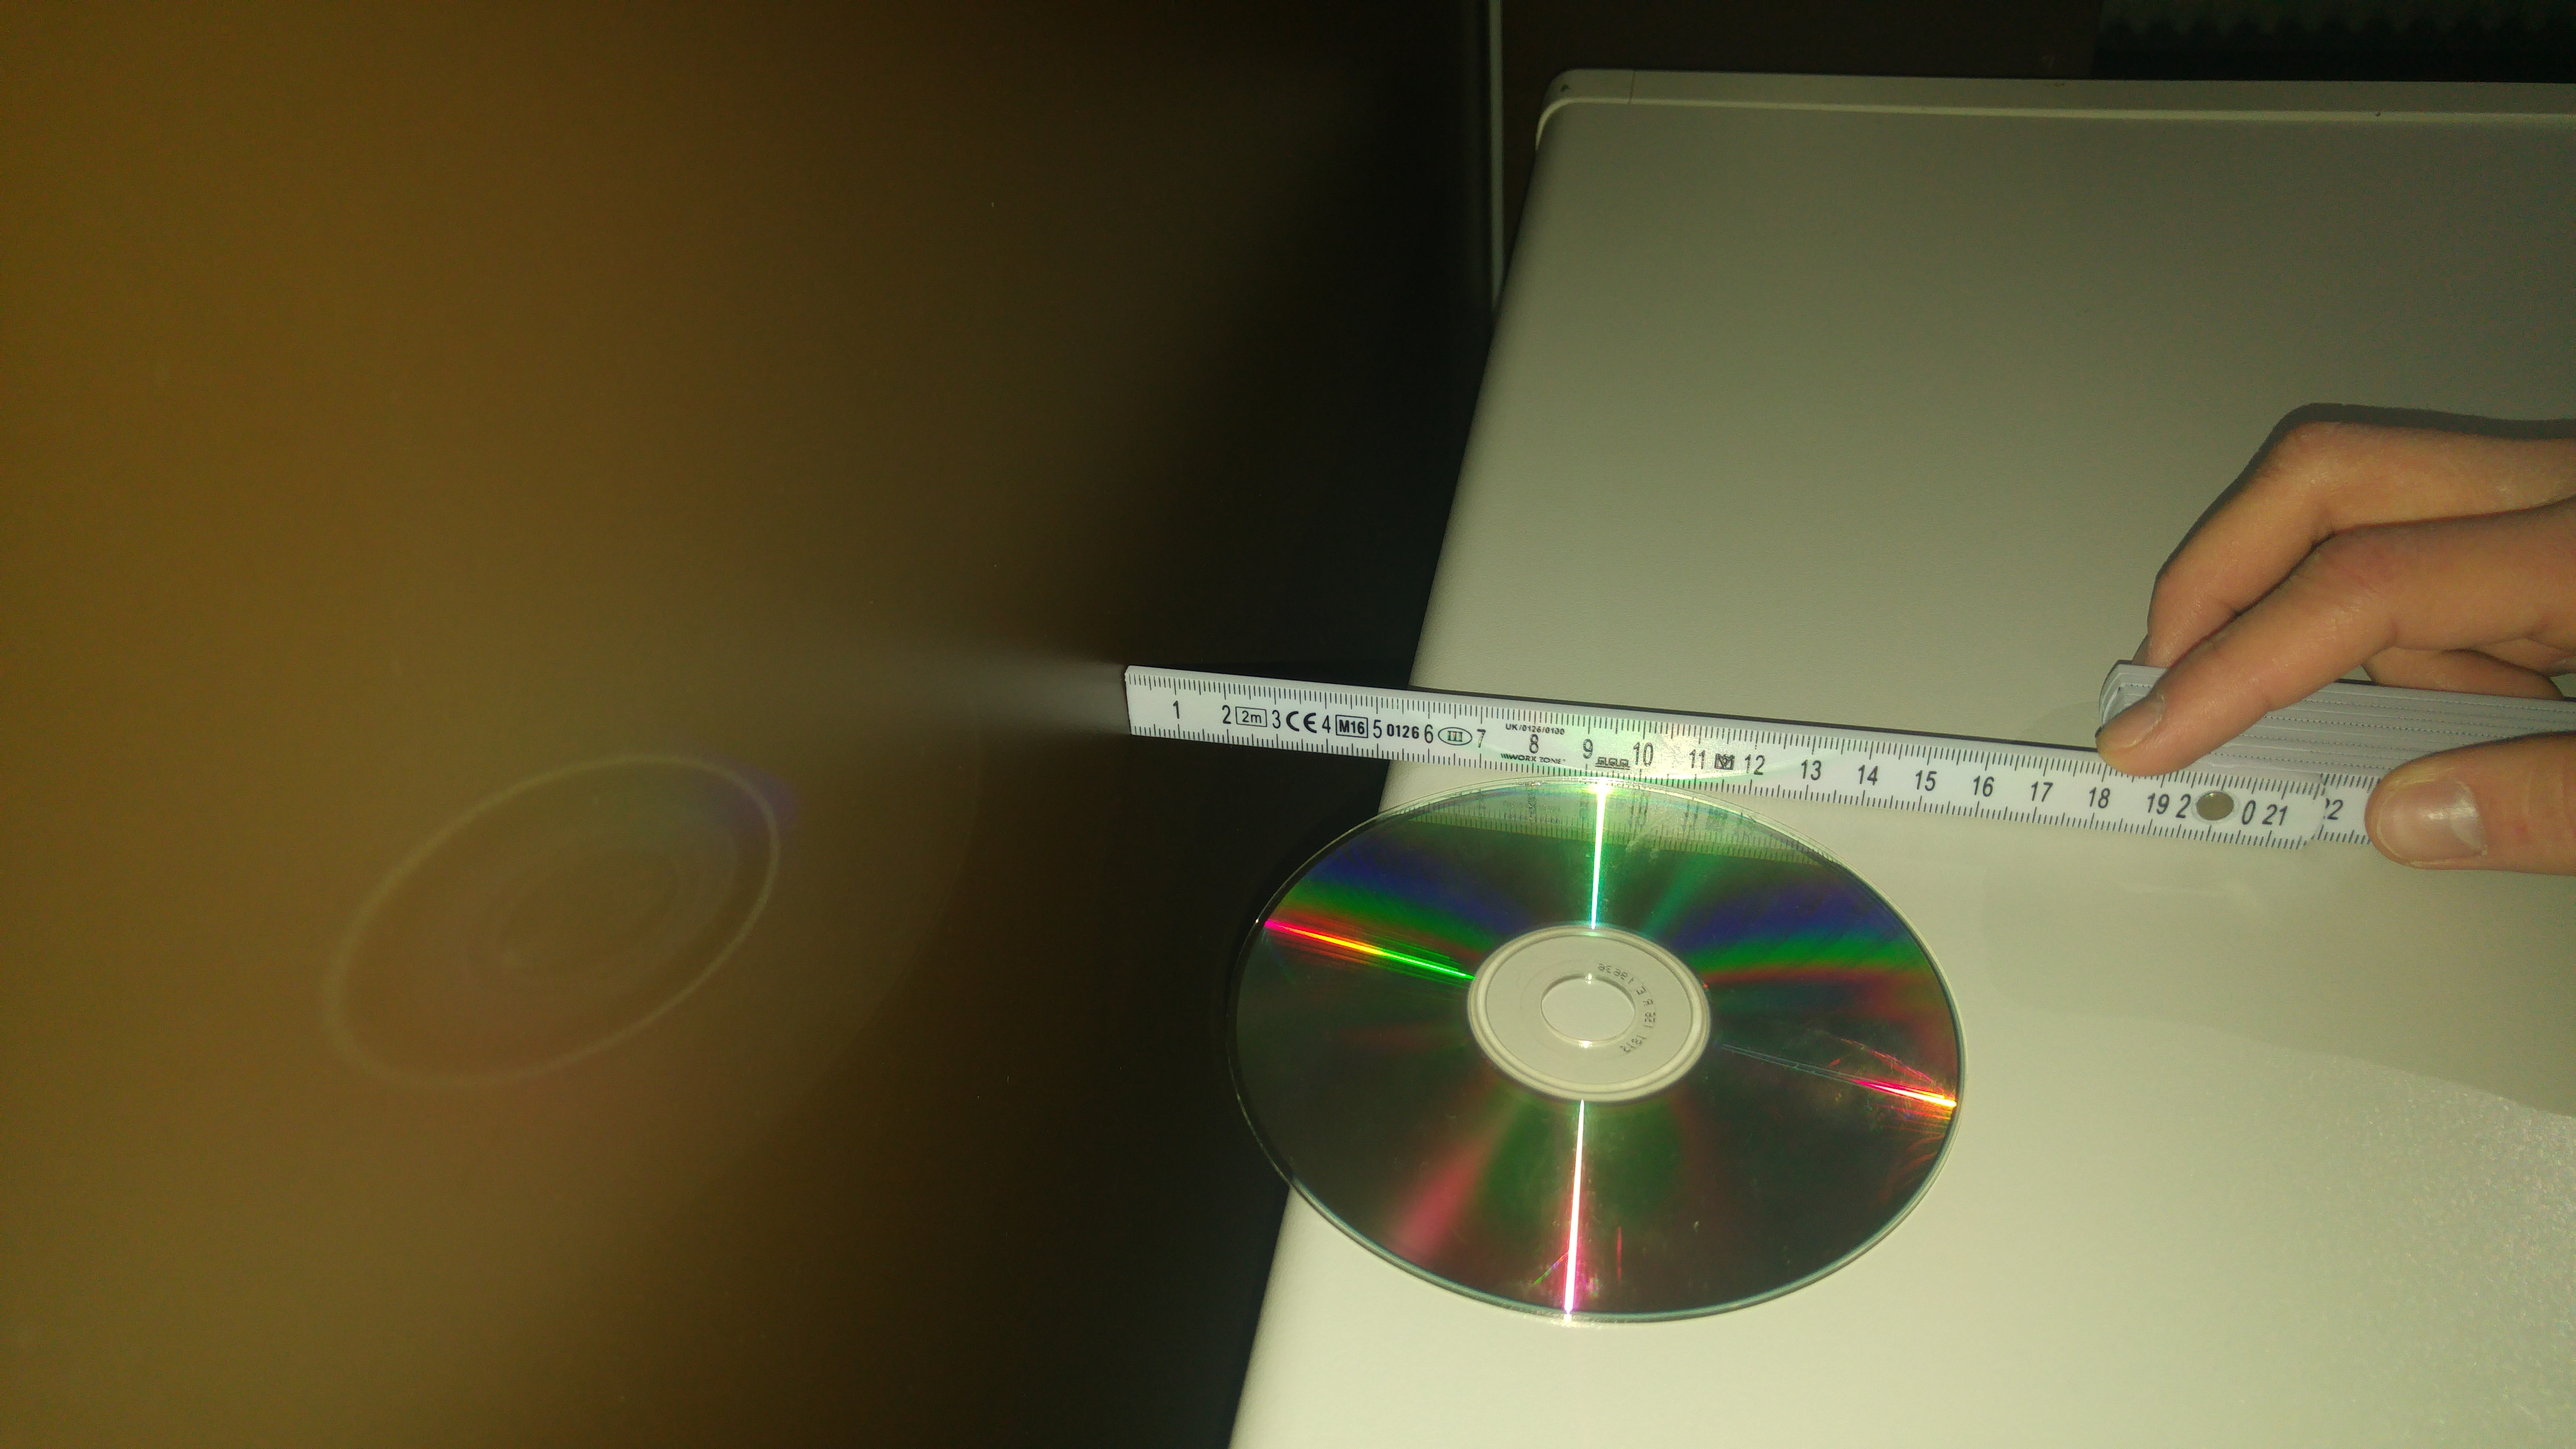
\includegraphics[width=0.6\textwidth,keepaspectratio]
{Pictures/20161219_142123.jpg}
\parbox{0.9\textwidth}

{\caption{\label{fig:Bild7}
Bildtitel für Bild 7}
\sffamily \small{Beschreibung für Bild 7}
}
\end{figure}

\begin{figure}[!htbp]
\centering
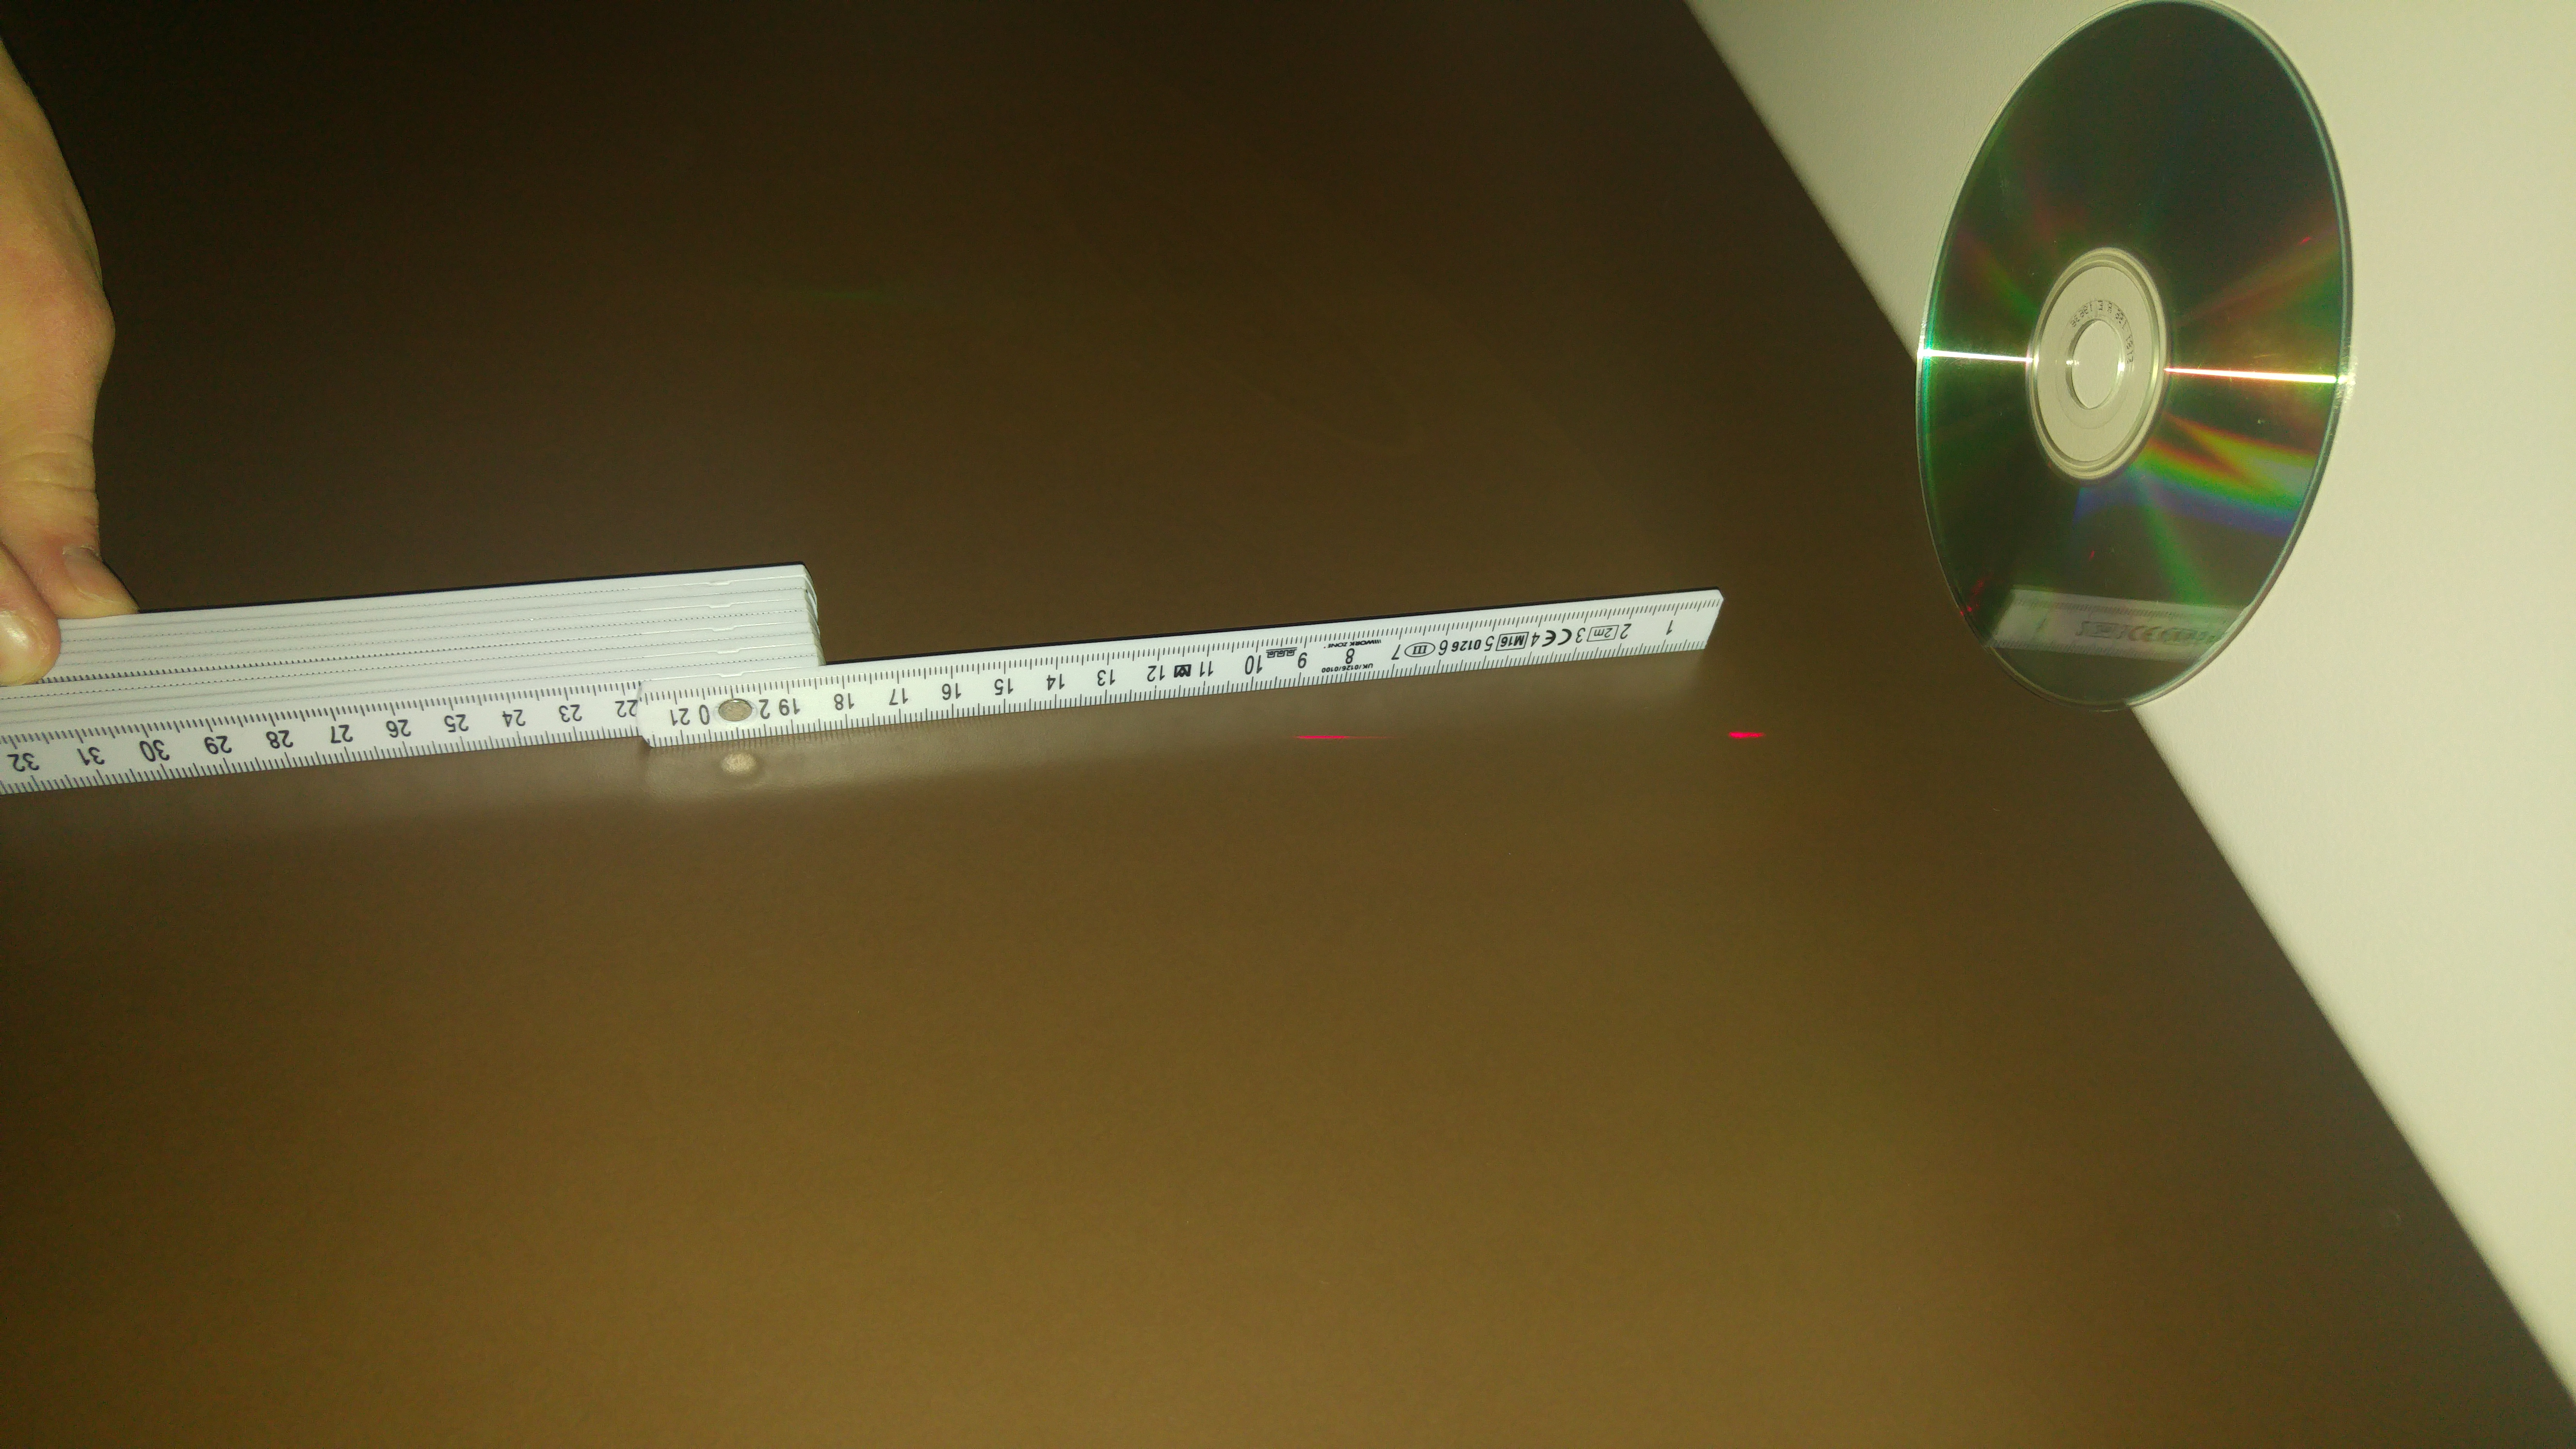
\includegraphics[width=0.6\textwidth,keepaspectratio]
{Pictures/20161219_142155.jpg}
\parbox{0.9\textwidth}

{\caption{\label{fig:Bild8}
Bildtitel für Bild 8}
\sffamily \small{Beschreibung für Bild 8}
}
\end{figure}

\begin{figure}[!htbp]
\centering
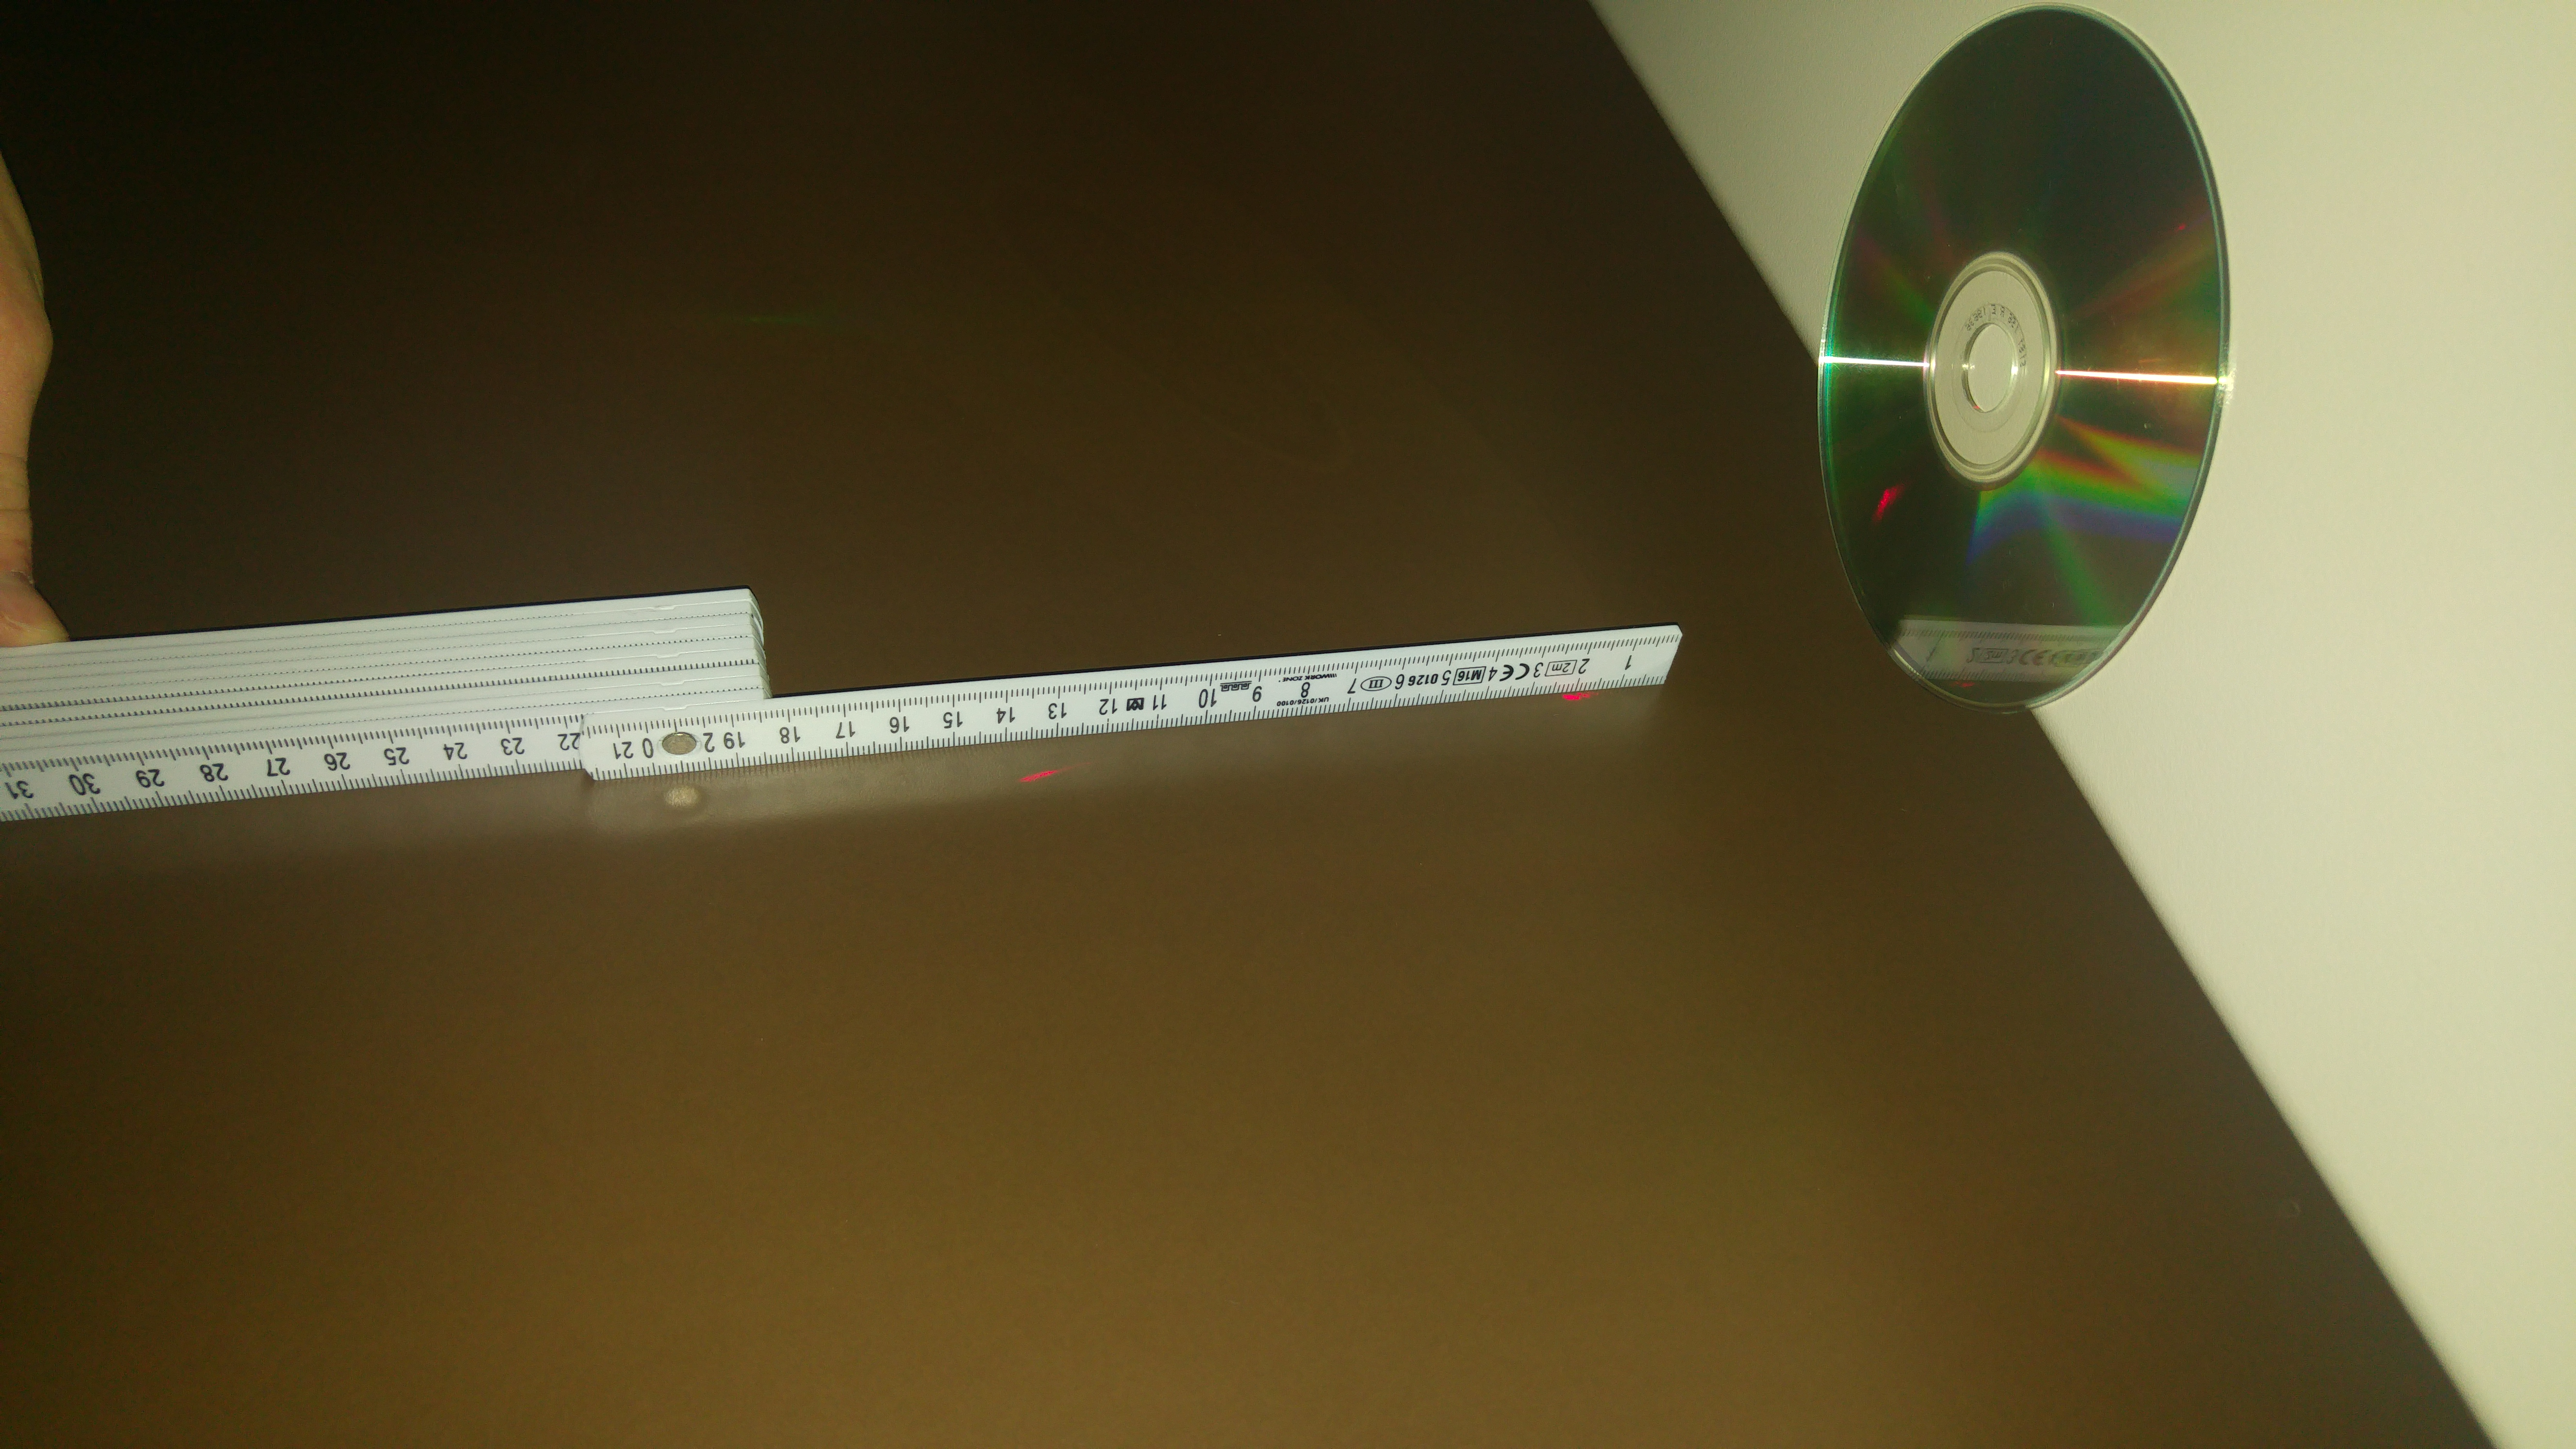
\includegraphics[width=0.6\textwidth,keepaspectratio]
{Pictures/20161219_142206.jpg}
\parbox{0.9\textwidth}

{\caption{\label{fig:Bild9}
Bildtitel für Bild 9}
\sffamily \small{Beschreibung für Bild 9}
}
\end{figure}

\begin{figure}[!htbp]
\centering
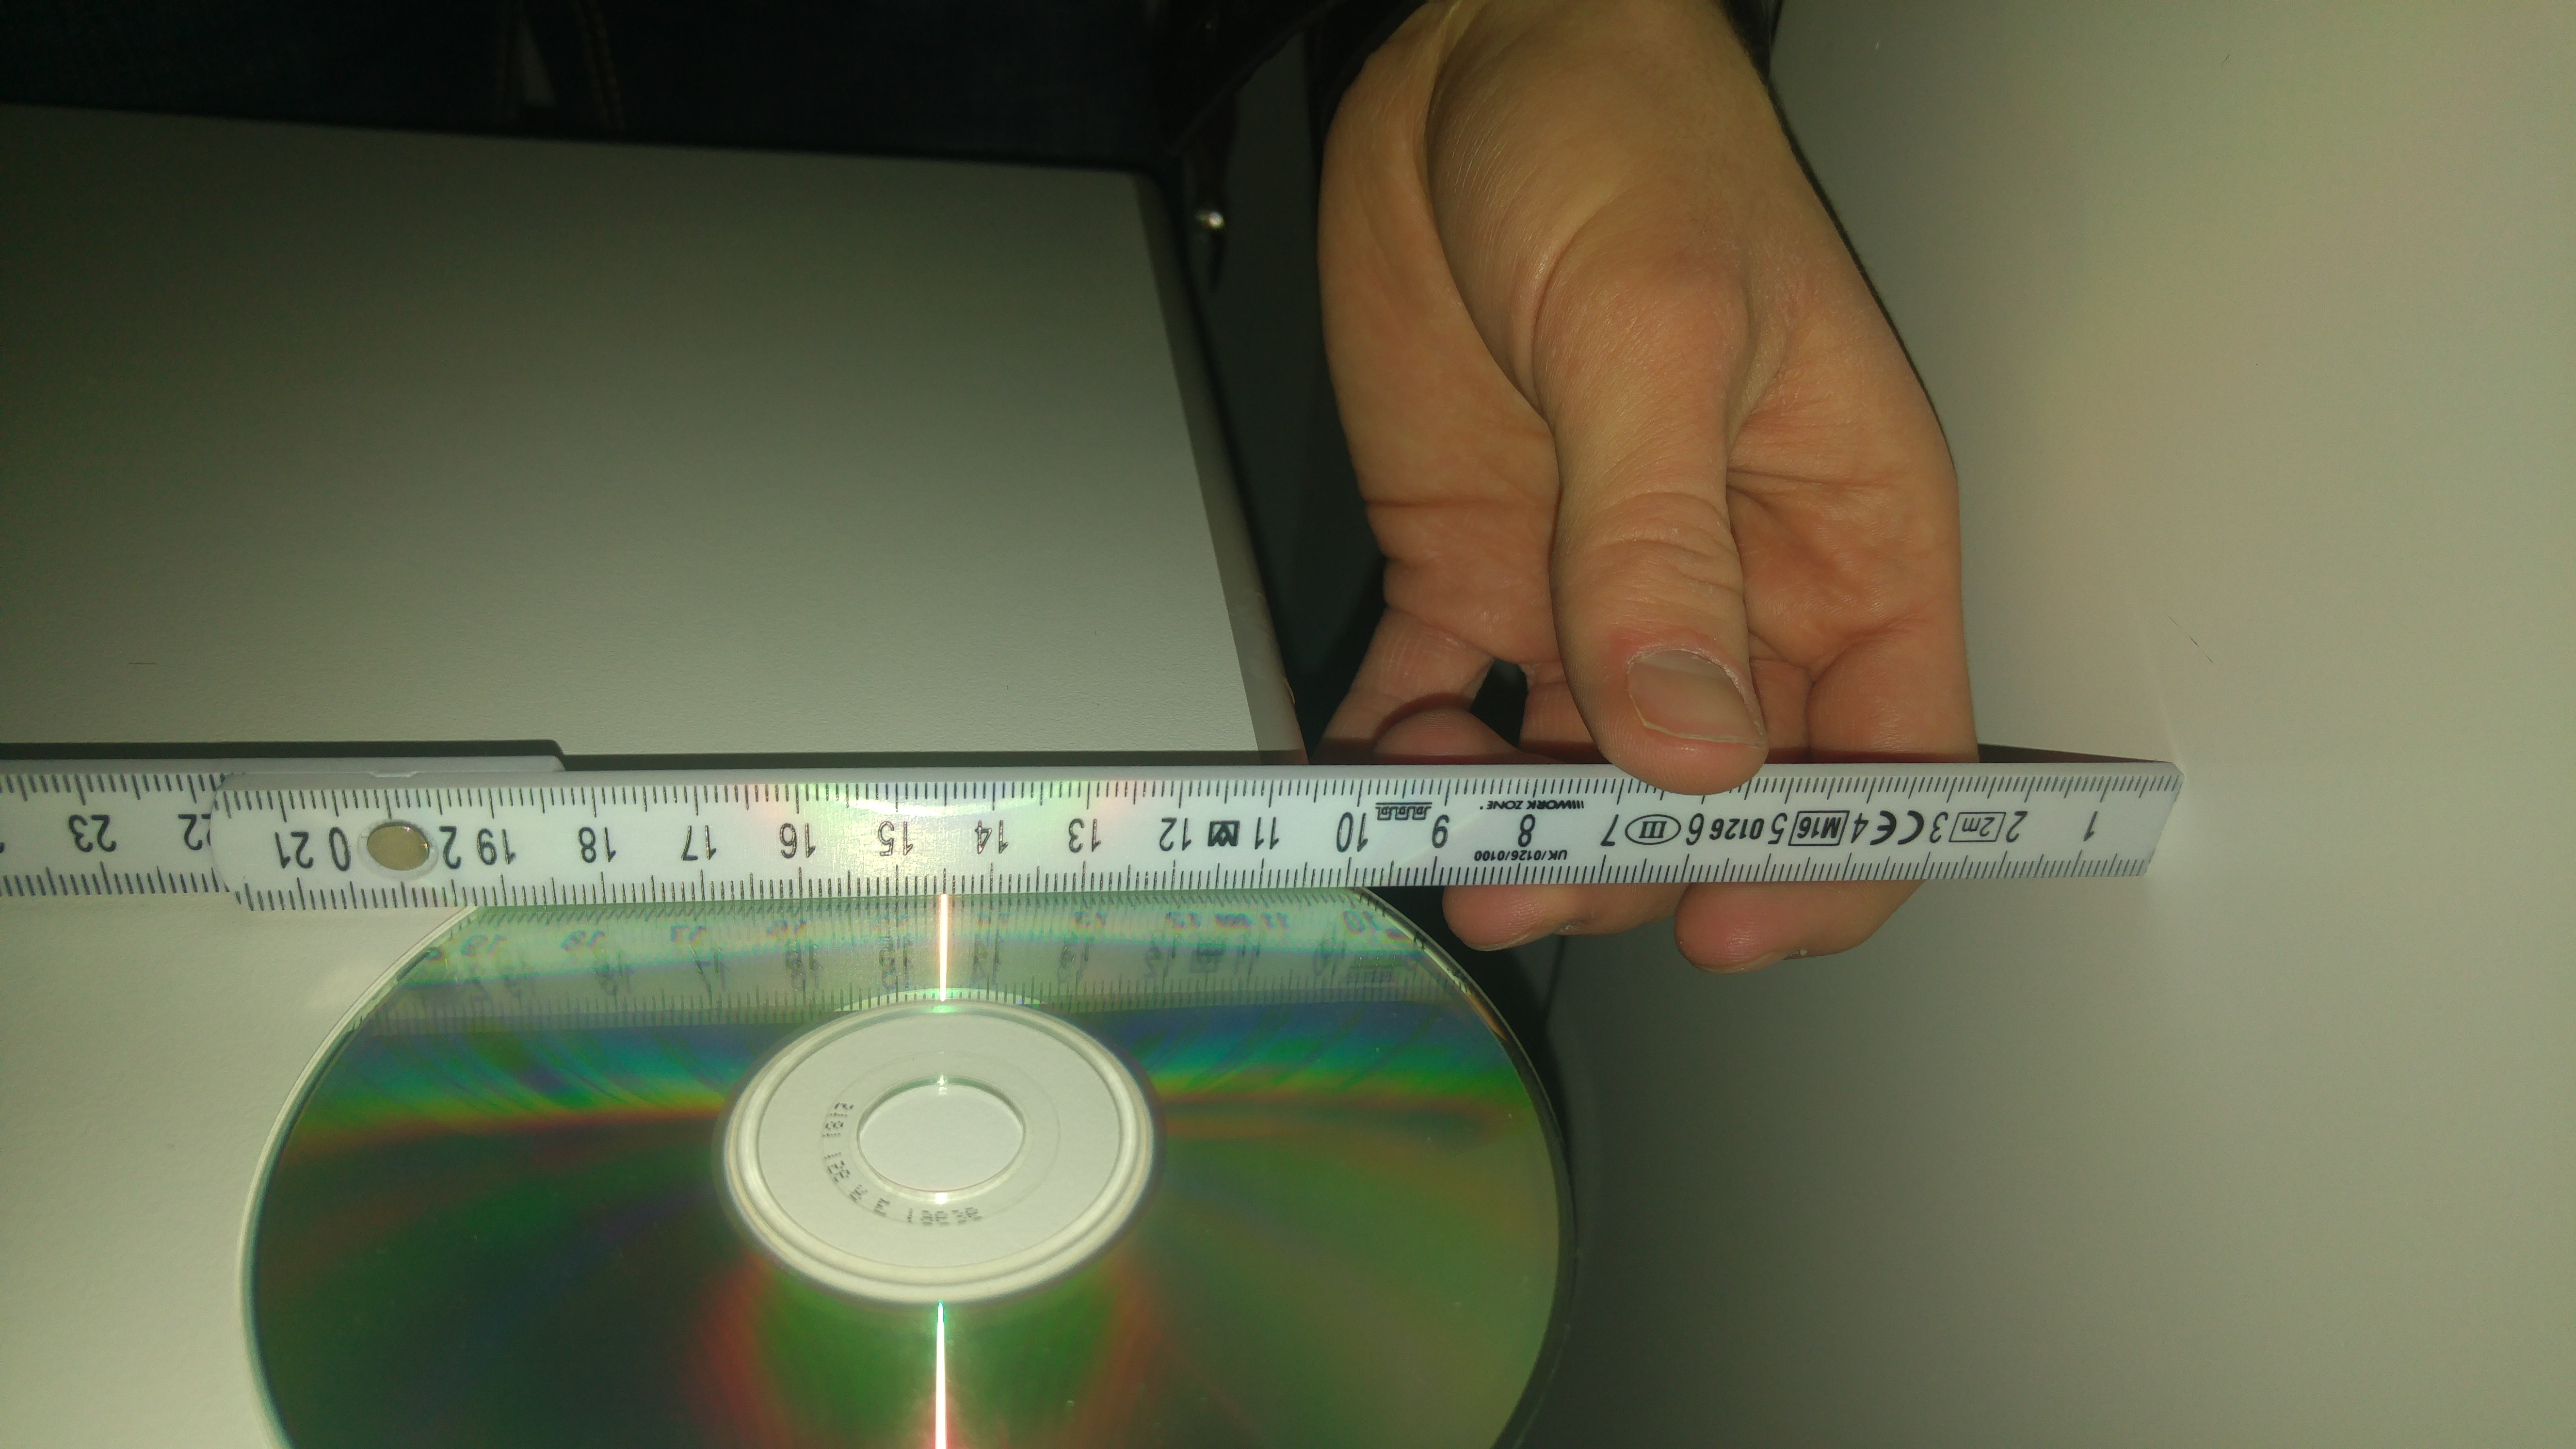
\includegraphics[width=0.6\textwidth,keepaspectratio]
{Pictures/20161219_144350.jpg}
\parbox{0.9\textwidth}

{\caption{\label{fig:Bild10}
Bildtitel für Bild 10}
\sffamily \small{Beschreibung für Bild 10}
}
\end{figure}

\begin{figure}[!htbp]
\centering
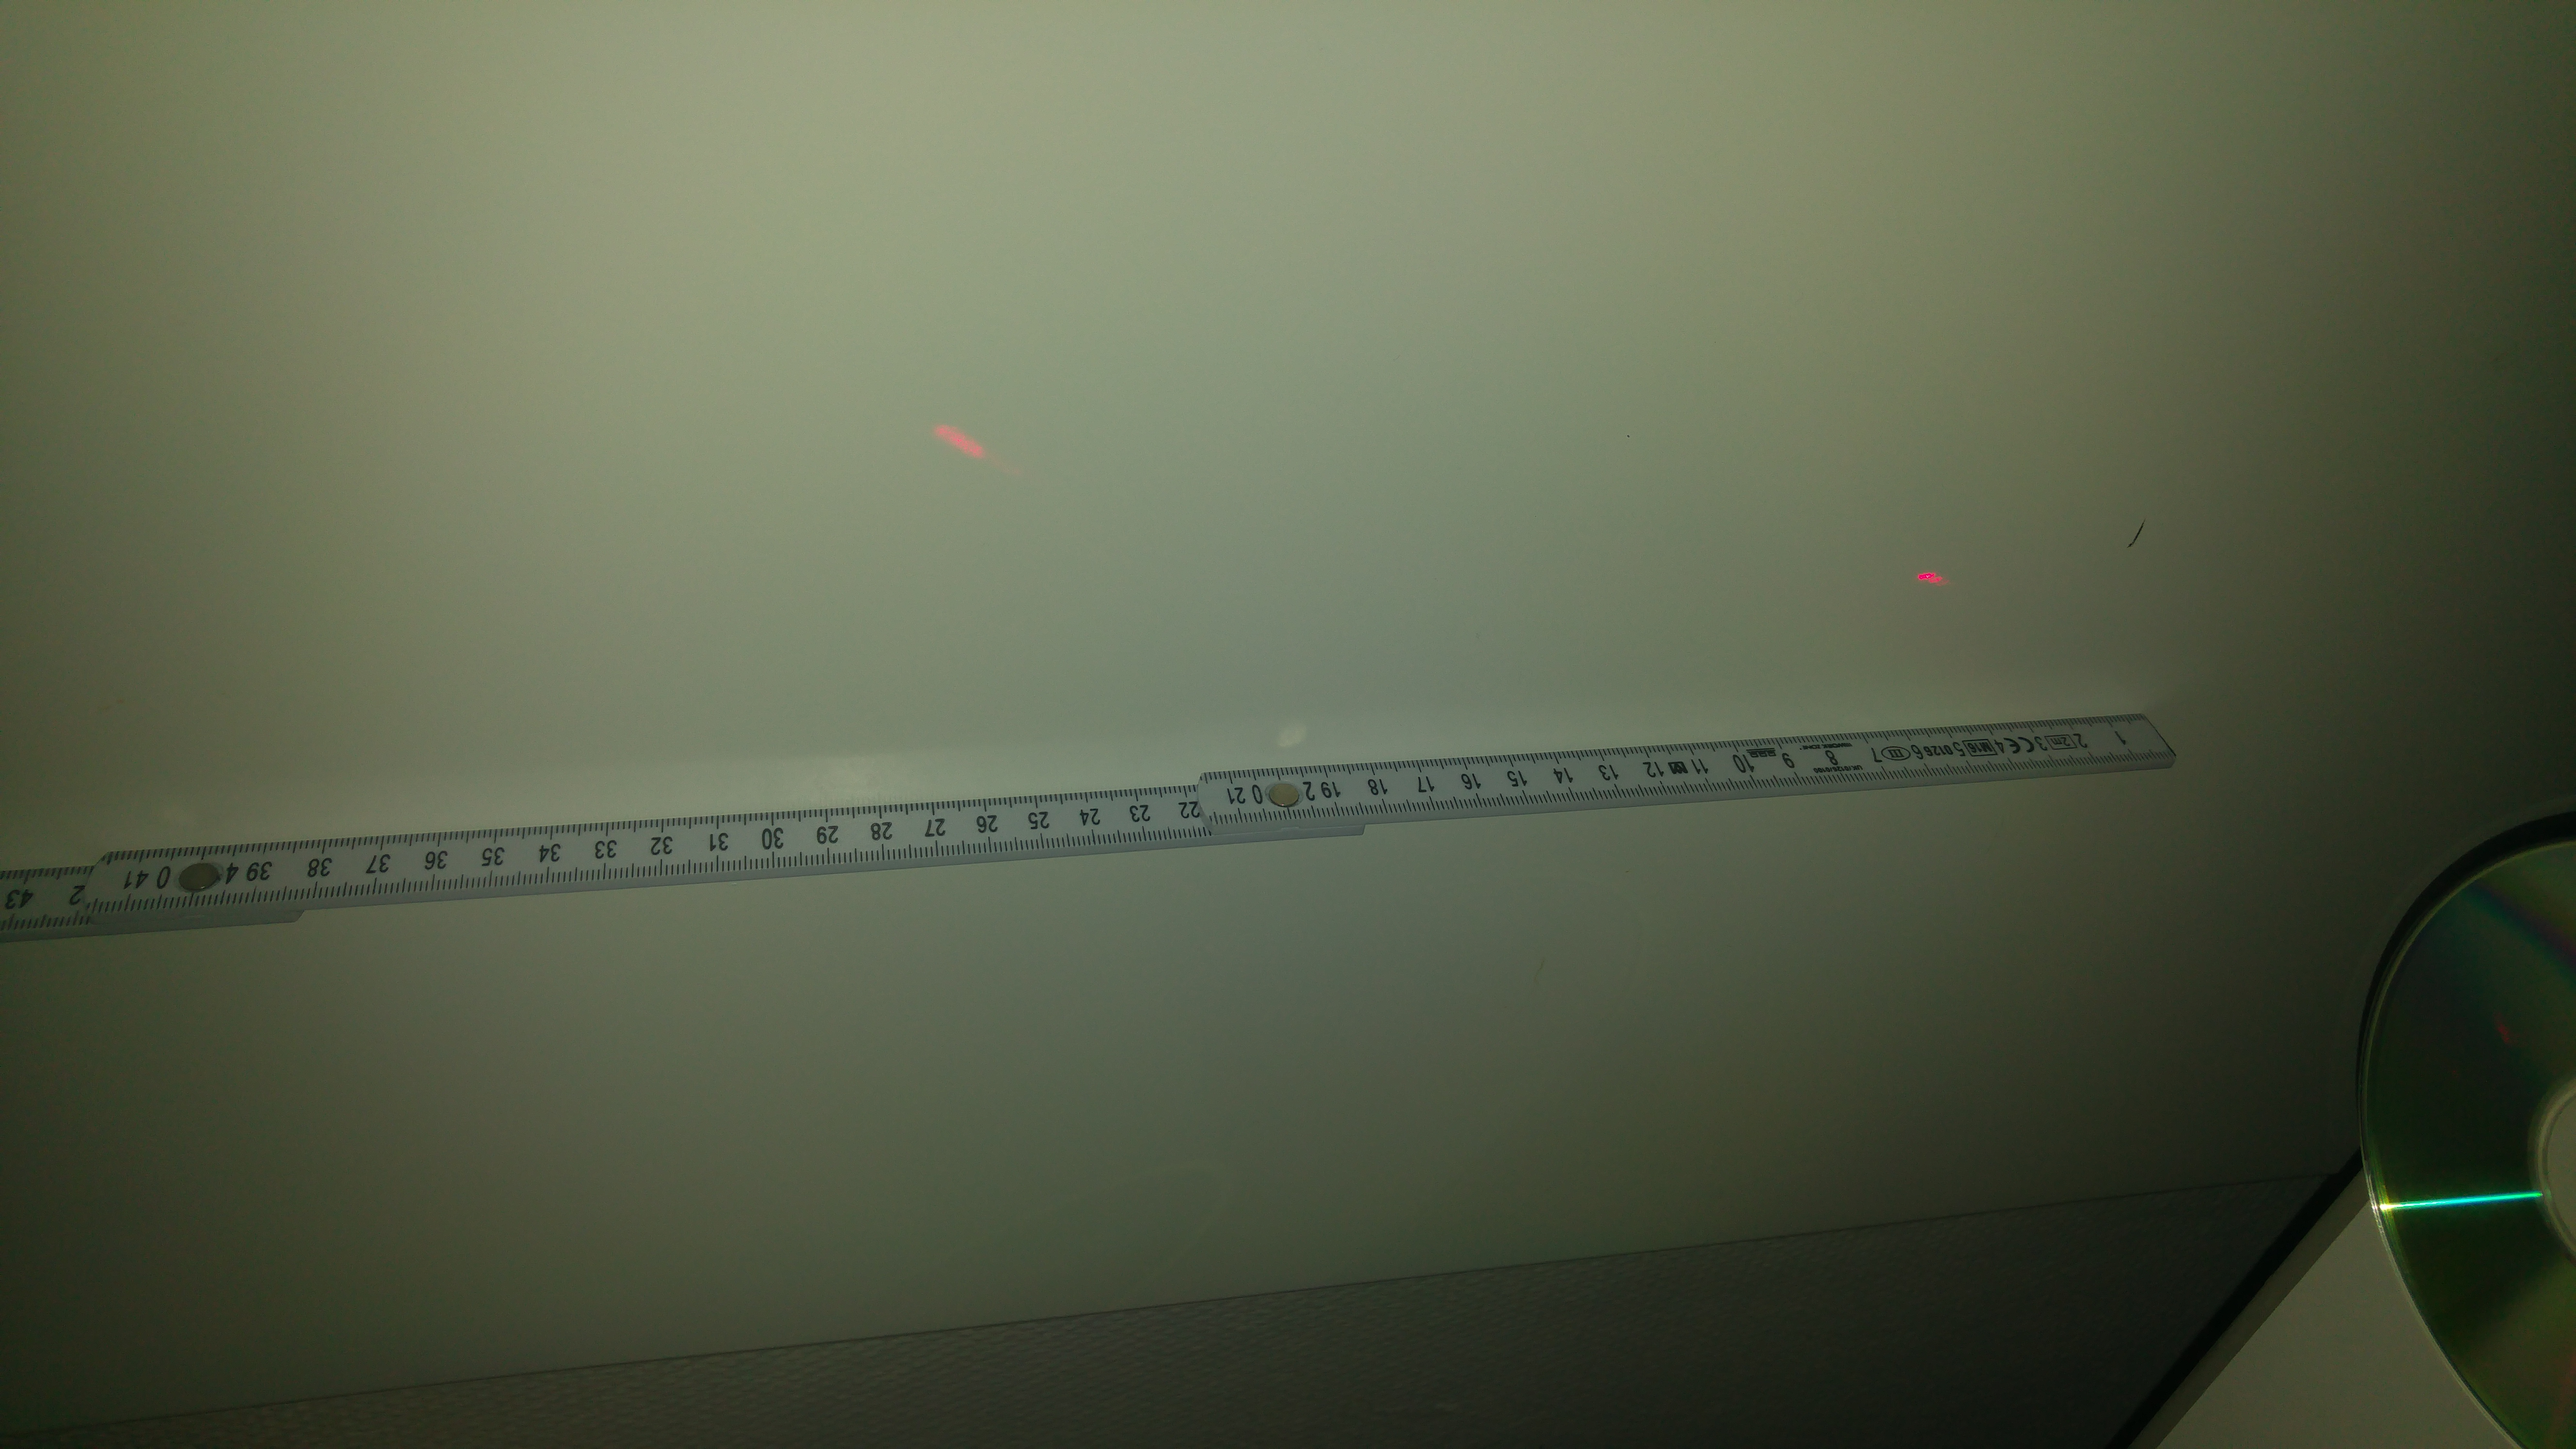
\includegraphics[width=0.6\textwidth,keepaspectratio]
{Pictures/20161219_144511.jpg}
\parbox{0.9\textwidth}

{\caption{\label{fig:Bild11}
Bildtitel für Bild 11}
\sffamily \small{Beschreibung für Bild 11}
}
\end{figure}

\begin{figure}[!htbp]
\centering
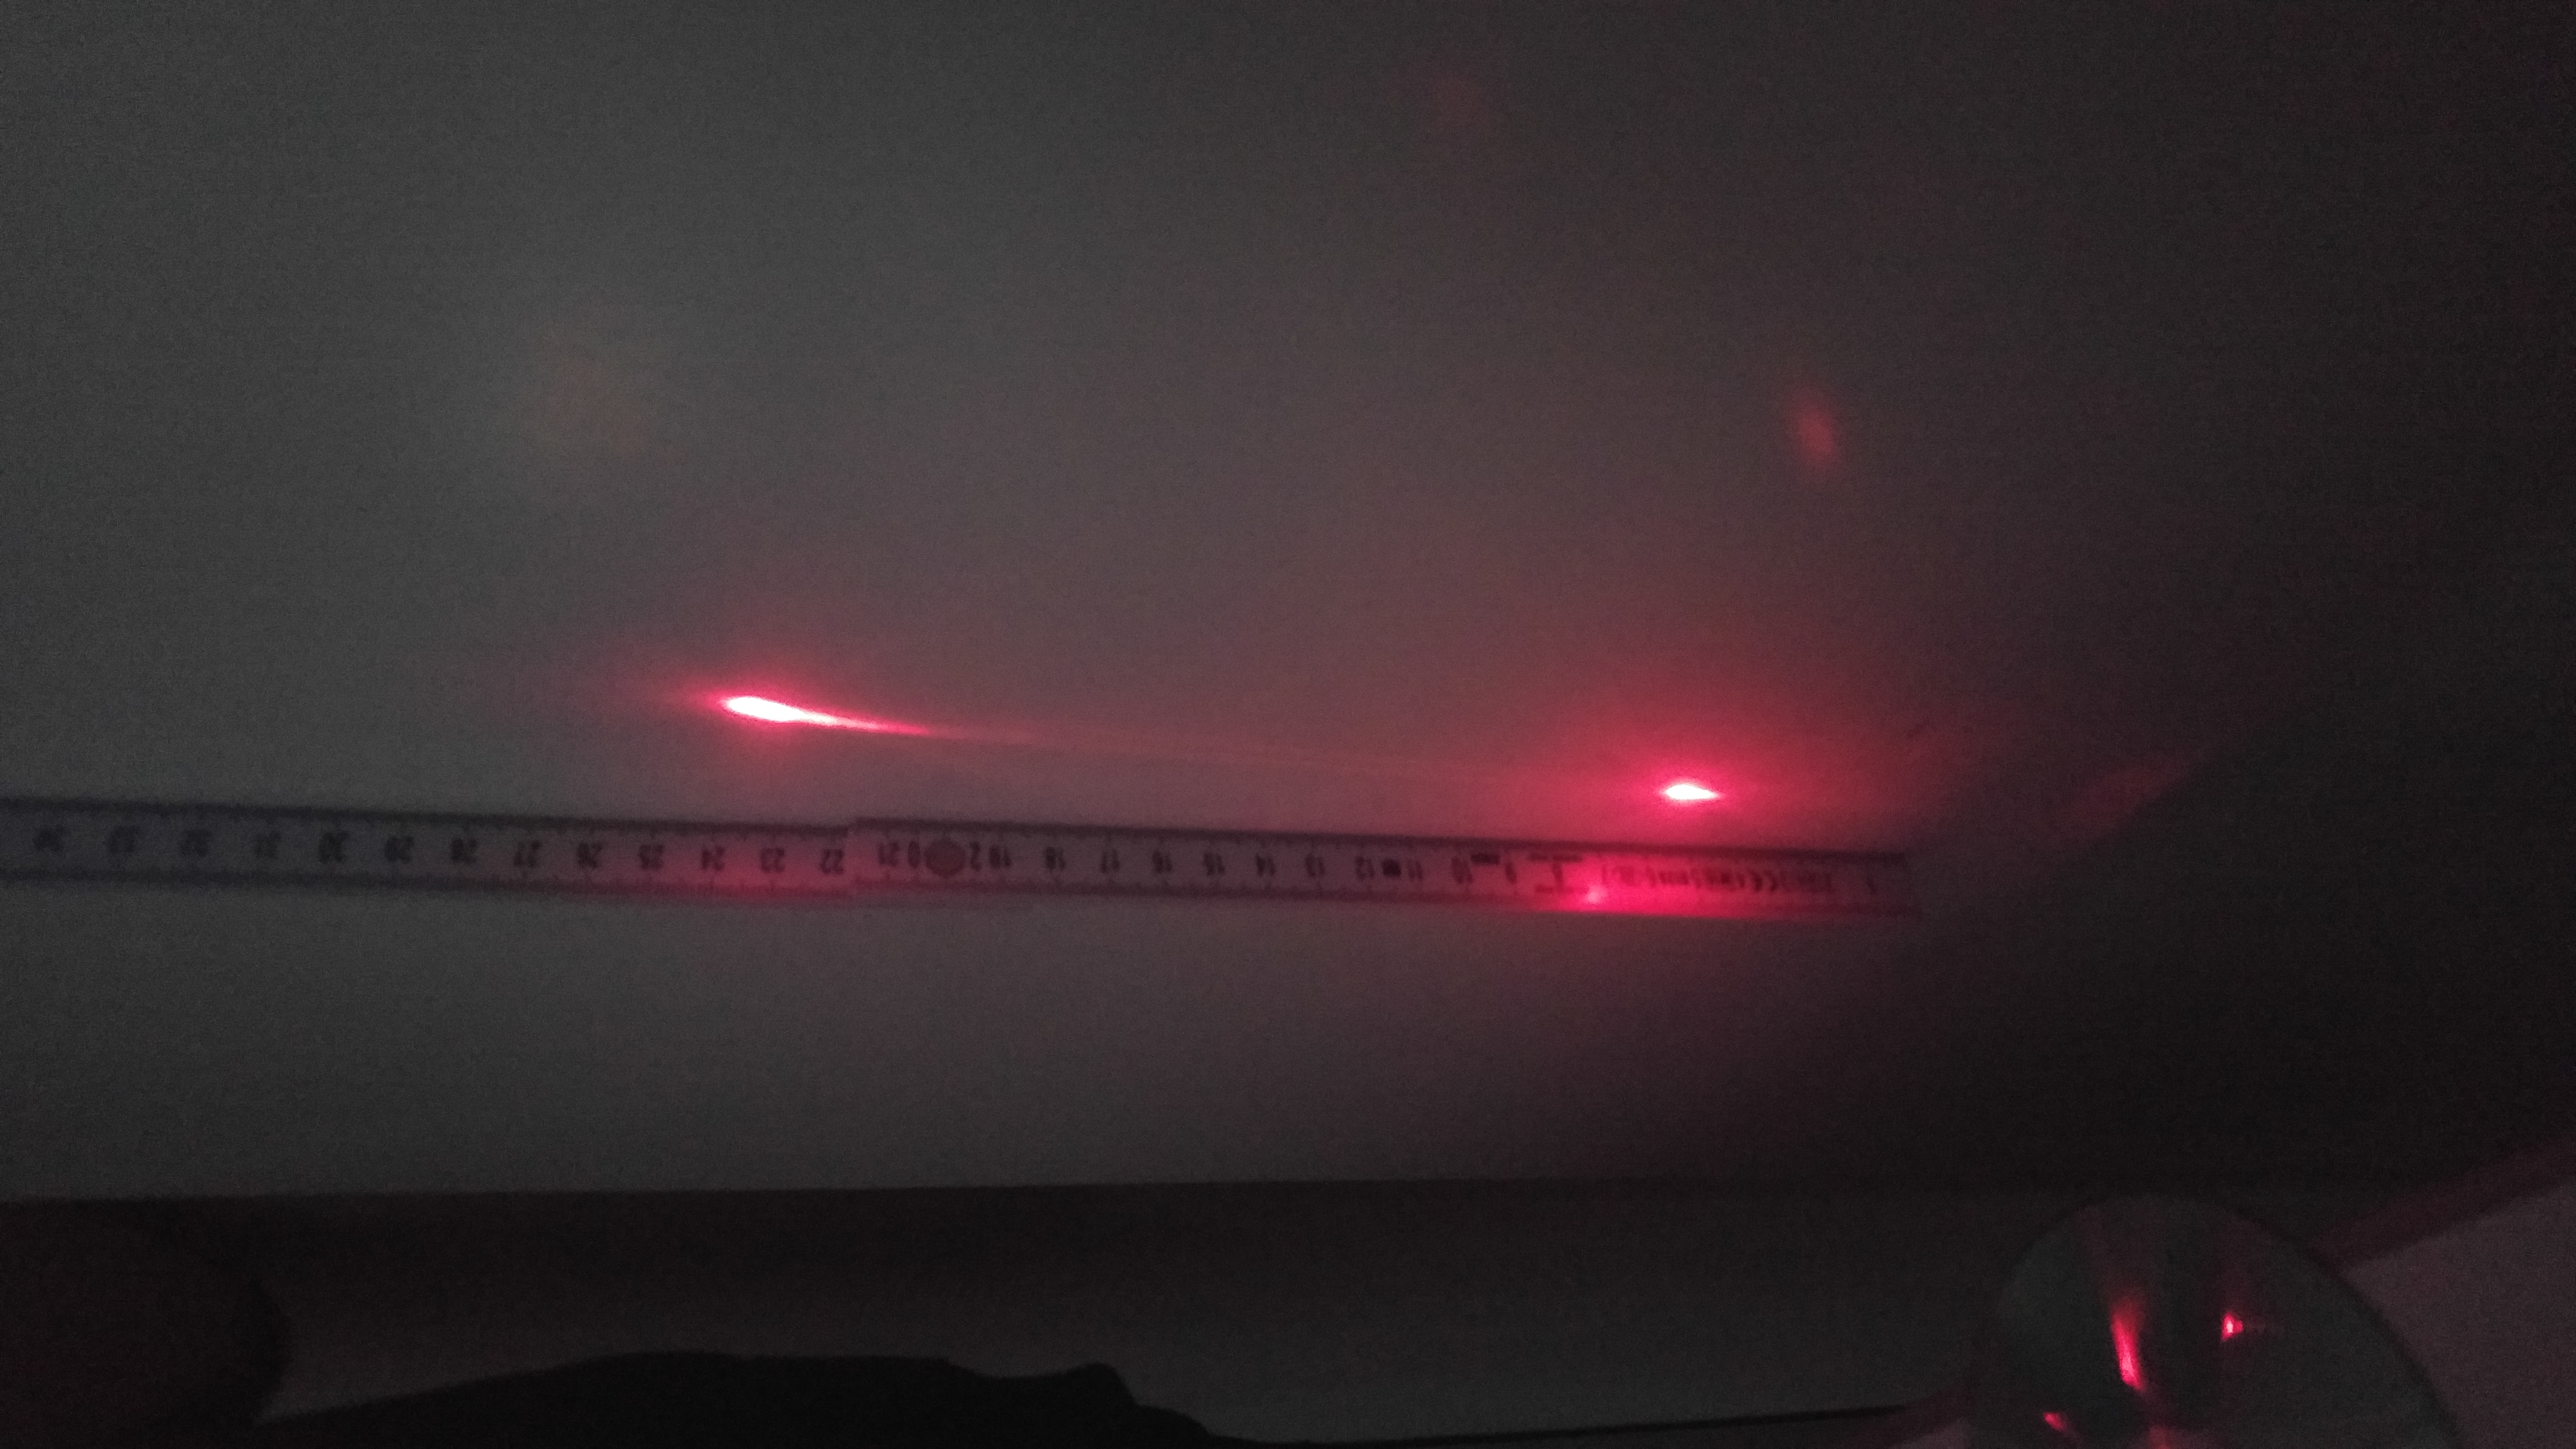
\includegraphics[width=0.6\textwidth,keepaspectratio]
{Pictures/20161219_144536.jpg}
\parbox{0.9\textwidth}

{\caption{\label{fig:Bild12}
Bildtitel für Bild 12}
\sffamily \small{Beschreibung für Bild 12}
}
\end{figure}


\end{document}